\documentclass[review]{igs}

\usepackage[T1]{fontenc}
\usepackage[utf8]{inputenc}
\usepackage{microtype}
\usepackage[english]{babel}
\usepackage{amsmath,amssymb,mathtools,bm}
\usepackage{booktabs,longtable}
\usepackage{graphicx}
\usepackage{enumitem}
\usepackage[authoryear,round]{igsnatbib}

\title[Isochrone overturning]{Isochrone overturning in steady glacier flow}
\author[Lipovsky]{Bradley Paul LIPOVSKY}
\affiliation{Department of Earth and Space Sciences, University of Washington, Seattle, USA\\
Correspondence: Bradley Paul Lipovsky, \texttt{bpl7@uw.edu}}

\begin{document}
\abstract{Ancient ice recovered at Allan Hills extends into the Miocene (\(23\)--\(5.3~\mathrm{Ma}\)), but steep layers, age reversals and folds complicate its interpretation. Whether steady glacier flow can overturn layers deposited in chronological order remains uncertain. Here, we track the horizontal order of particles deposited sequentially at the surface. This order is measured by a signed Jacobian that is equivalent to the inverse vertical-thinning factor while layers remain ordered. We find that overturning depends directly on the cumulative competition between vertical shear, which preserves depositional order, and reverse shear, which erodes it. Reverse shear accumulates faster where horizontal speed is small. Because a layer becomes vertical only after reverse shear has erased both its initial ordering and the ordering accumulated during earlier upstream flow, local flow alone cannot estimate stratigraphic overturning. The Stokes equations supply no general sign-preservation result, although shallow-ice flow under a strictly downhill surface slope does. We derive an overturning threshold, bounds for localized obstacles, a cancellation result for periodic bed roughness and trajectory-based diagnostics for numerical models. For both linear-viscous and nonlinear Glen (\(n=3\)) rheologies, a finite convergent point-margin Stokes flow reverses an ordered incoming material line under its stated boundary closure, whereas 750 linear-viscous and 745 nonlinear Glen periodic sinusoidal-bed calculations preserve surface-deposition order. Layer curvature and topographic draping can occur without order reversal; the Jacobian provides a theoretical test for evaluating steady-flow explanations of disturbed stratigraphy at Allan Hills and other old-ice sites.}

\maketitle

\noindent\textbf{Keywords:} glacier flow; ice stratigraphy; recumbent folds; blue ice; Stokes modelling

\section{Introduction}

Recovering old ice is most useful where its age and stratigraphic context can be established. At Little Dome C, radar and flow modelling have been used to target a continuous record beyond \(1~\mathrm{Ma}\) \citep{Lilien2021,Chung2025BeyondEPICA}. Antarctic blue-ice areas instead expose discontinuous intervals through surface ablation and upward ice motion \citep{Bintanja1999,Spaulding2012}. The S{\o}r Rondane Mountains are another blue-ice setting being surveyed for old ice \citep{Izeboud2026}. At Allan Hills, cores have progressed from disturbed ice near \(1~\mathrm{Ma}\) to Pliocene (\(5.3\)--\(2.6~\mathrm{Ma}\)) and Miocene (\(23\)--\(5.3~\mathrm{Ma}\)) ice and air approaching \(6~\mathrm{Ma}\) \citep{Higgins2015,Yan2019,Shackleton2025}.

Allan Hills ice is locally out of order: ALHIC1901 contains multiple age reversals \citep{Shackleton2025}; two recent cores have mean layer dips of approximately \(29^{\circ}\) and \(69^{\circ}\) \citep{Kirkpatrick2025}; and ALHIC1901 microstructure records simple shear, crystal-orientation stripes and centimetre-scale folds \citep{Stoll2026}. Radar and flow modelling show strong spatial variation in archive continuity and transport history \citep{Kehrl2018,Manos2026}. Layer deformation therefore affects the interpretation of the recovered ages.

ALHIC1901 and ALHIC1902 lie only \(1.5~\mathrm{km}\) apart but sample different local flow regimes. ALHIC1901 lies in faster flow across a buried extension of the nunatak, whereas ALHIC1902 lies beside the nunatak in a modelled zone of slow basal flow \citep{Manos2026}. Their \(^{40}\mathrm{Ar}_{\mathrm{atm}}\) chronologies are nonmonotonic with depth (Figure~\ref{fig:allan-hills-context}): ALHIC1901 contains several metre-scale decreases in age with increasing depth, and ALHIC1902 contains a resolved reversal between approximately \(142\) and \(145~\mathrm{m}\) \citep{Shackleton2025,MarksPeterson2026}. These age reversals are a direct core-scale signature of disturbed order. They imply an overturned continuous isochrone only where the samples belong to one continuous surface-deposited layer family.

\begin{figure}[t]
\centering
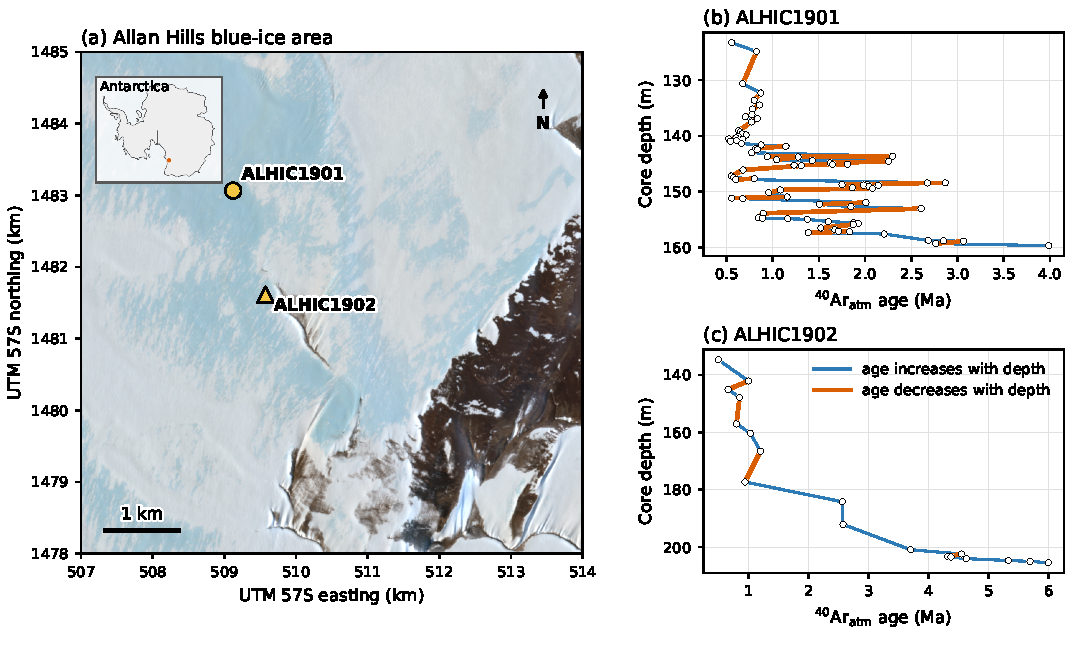
\includegraphics[width=\textwidth]{../figures/allan_hills_context.pdf}
\caption{Allan Hills setting and published age--depth reversals. (a) Contrast-enhanced \(10~\mathrm{m}\) Copernicus Sentinel-2 L2A image acquired on 30 December 2025, with the locations of the two cores whose chronologies are plotted at right. The inset locates Allan Hills in Antarctica. (b) ALHIC1901 \(^{40}\mathrm{Ar}_{\mathrm{atm}}\) ages used in Figure~1b of \citet{MarksPeterson2026}. (c) ALHIC1902 \(^{40}\mathrm{Ar}_{\mathrm{atm}}\) ages from \citet{Shackleton2025}. Curves connect measurements in order of increasing depth; orange segments mark intervals where reported age decreases with depth. A decrease in age with depth establishes nonmonotonic core stratigraphy, but it implies an overturned continuous isochrone only if the samples belong to one continuous surface-deposited layer family. Core coordinates are from \citet{Shackleton2025}.}
\label{fig:allan-hills-context}
\end{figure}

It remains unclear whether fixed topography in a steady glacier can generate a recumbent fold. Flow over topography produces layer draping or overriding \citep{Hindmarsh2006}, while rough-bed Stokes solutions can contain local extrusion (i.e., faster flow at depth) or, at greater slopes, separated circulation \citep{Gudmundsson1997linear,Gudmundsson1997nonlinear,Waddington2010}. Whether these motions reverse stratigraphic order is less clear.

Structural geology makes a related distinction between active competence-driven buckling and passive amplification of layers in heterogeneous shear, either of which can produce recumbent or sheath folds in rocks \citep{Bastida2014,SchmalholzMancktelow2016,NabaviFossen2021}. Field and fabric analyses show that sheath folds often combine early active folding with subsequent passive shear and hinge rotation \citep{Fazio2024,AlsopCondon2025}. Whereas rock-folding analyses follow pre-existing layers, glacier stratigraphy is generated continuously at the surface during flow. In glaciers, \citet{Hudleston1976} similarly attributed Barnes Ice Cap folds to flow changes during minor advances or retreats, followed by bed-related shear, while \citet{WhillansJohnsen1983} reproduced Byrd Station layer undulations using steady linear-viscous flow over basal variations without obtaining recumbent order reversal.

Airborne radar and deep ice cores show that order-reversing structures occur at ice-sheet scale. In the NEEM ice core, \citet{DahlJensen2013} reconstructed the Eemian interglacial climate record from folded basal ice using chronological markers to unwrap stratigraphic inversions. Dated radar horizons at Petermann Glacier contain overturned limbs and a sheath fold \citep{Bons2016}. Three-dimensional radar mapping in northeast Greenland resolved \(500\)--\(600~\mathrm{m}\) overturned anticline--syncline pairs associated with extinct ice streams \citep{Franke2022}. \citet{Franke2022} interpreted these structures as upright folds formed by earlier convergent flow and subsequently sheared into recumbent geometries after flow reorganization.

\citet{Waddington2001} examined whether local shear rotates a pre-existing wrinkle toward overturning or whether longitudinal extension flattens it, and argued that a transient process must first disturb steady stratigraphy. Finite-strain calculations later followed such inherited disturbances along trajectories and showed how divide migration can supply them \citep{JacobsonWaddington2004,JacobsonWaddington2005}. For continuously generated steady stratigraphy, \citet{ParreninHindmarshRemy2006} introduced logarithmic flux coordinates, and \citet{ParreninHindmarsh2007} generalized this construction to horizontally non-uniform velocity. Their \((\pi,\theta)\) coordinates (see Table~\ref{tab:notation} in Appendix~\ref{app:notation} for notation)---the logarithms of total flux and normalized streamfunction---make steady particle trajectories parallel straight lines labelled by their surface origin \(\pi_0\). The associated path-sign parameter \(\alpha\) measures the change in separation between neighboring surface origins and shows that an isochrone passes through vertical when \(\alpha>1\). They proved that upward-increasing horizontal velocity precludes this state, but did not construct a glacier flow with \(\alpha>1\) or connect the criterion to Stokes mechanics. Their framework also supports vertical thinning functions and numerical age solvers \citep{Parrenin2013,HindmarshLeysingerVieliParrenin2009,ParreninChungMartin2025}.

Steady accumulation and near-surface flow can produce single-valued firn undulations \citep{NgKing2011,NgKing2013}, whereas traveling basal-traction anomalies produce overturned folds through an explicitly transient mechanism \citep{Wolovick2014,WolovickCreyts2016}. Non-Newtonian normal-stress differences can drive secondary spiral flows in basal ice \citep{SchoofClarke2008}, and Stokes models also amplify seeded or active structures through anisotropy, basal shear and bed relief \citep{Zhang2024}. Not every fold-like radar return traces a continuous surface-deposited isochrone. Steep specular limbs may be poorly imaged \citep{Holschuh2014}, and some northern Greenland structures contain debris-rich horizons with diffuse scattering \citep{Holschuh2026}. The unresolved step is whether a steady glacier velocity field can overturn the passive age field generated continuously at the surface. Table~\ref{tab:lineage} (Appendix~\ref{app:lineage}) summarizes the relationship between these studies and the present analysis.

Here, we treat age as a passive, non-diffusive scalar introduced at surface deposition, and write the signed inverse vertical-thinning factor as the horizontal order of particles along an isochrone. Its cumulative budget separates surface-fast regular shear and extrusive reverse shear. We relate that budget to the Stokes stress balance, derive preservation regimes and obstacle bounds, and formulate trajectory diagnostics. We then apply the direct tangent diagnostic to an incoming material line in a finite point-margin flow and to surface-deposited layers over periodic sinusoidal beds using both linear-viscous and nonlinear Glen (\(n=3\)) ice rheologies.

\section{Steady age transport and the order Jacobian}

\subsection{Physical question, governing equations and material origin}

Consider two neighboring ice parcels deposited sequentially at the surface of a steady two-dimensional glacier, at horizontal positions \(x_0\) and \(x_0+\delta x_0\) with \(\delta x_0>0\), and advected by the flow for the same elapsed time. Does the parcel deposited farther downstream remain downstream of its neighbor? We refer to this horizontal spatial sequence of parcels along an equal-age surface (isochrone) as \emph{stratigraphic order}, distinct from the stratigraphic age \(\tau\) itself. Curvature alone does not indicate overturning, because a strongly curved isochrone can remain a single-valued depth surface and preserve the depositional sequence. Rather, stratigraphic order is measured directly by the signed \emph{isochrone-order Jacobian},
\begin{equation}
\mathcal{J}(x,x_0)
=\left.\frac{\partial x}{\partial x_0}\right|_{\tau},
\label{eq:Jdefinition}
\end{equation}
where \(x\) is the present horizontal position of a parcel on the isochrone of age \(\tau\). Order is preserved while \(\mathcal{J}>0\), a vertical tangent forms where \(\mathcal{J}=0\), and an overturned limb corresponds to \(\mathcal{J}<0\) (Figure~\ref{fig:geometry}).

Integrating horizontal velocity along individual pairs of trajectories can test whether two parcels swap order in a given numerical velocity field, but it does not identify which dynamical terms in the flow field cause overturning, yield analytical preservation bounds or connect directly to the vertical age gradient measured in an ice core. The goal of this section is to express \(\mathcal{J}\) analytically in terms of the velocity field encountered along a trajectory using streamfunction--age coordinates.

\begin{figure}[t]
\centering
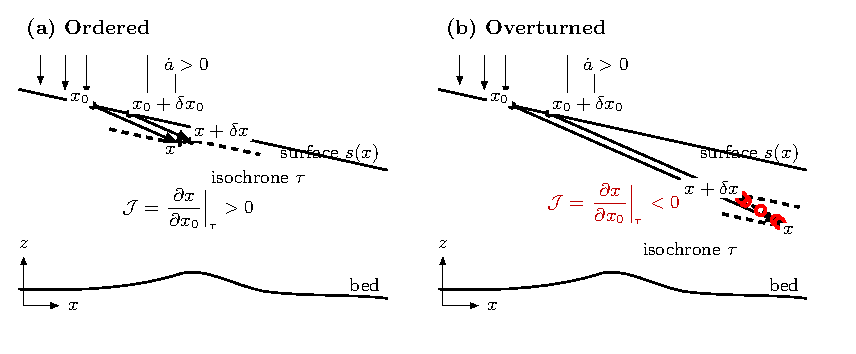
\includegraphics[width=\textwidth]{../figures/Figure1.pdf}
\caption{Material map for steady plane flow illustrating the three regimes of stratigraphic order. In each panel, neighboring parcels enter through the surface accumulation zone (\(\dot a>0\)) at \(x_0\) and \(x_0+\delta x_0\), follow distinct streamlines and reach positions \(x\) and \(x+\delta x\) on an equal-age surface (isochrone of age \(\tau\)); the order Jacobian is the limit \(\mathcal{J}=\lim_{\delta x_0\to 0}\delta x/\delta x_0\). (a) Ordered stratigraphy (\(\mathcal{J}>0\), \(\delta x>0\)). (b) Vertical tangent (\(\mathcal{J}=0\), \(\delta x/\delta x_0\to 0\)), marked by the vertical dotted line. (c) Overturned limb (\(\mathcal{J}<0\), \(\delta x<0\)), highlighted in red, where the parcel deposited at \(x_0+\delta x_0\) lies upstream of the parcel deposited at \(x_0\). The curves are plotted from an exact incompressible kinematic map satisfying surface origin, positive accumulation, non-intersecting streamlines and transverse intersections with the isochrone, rather than a calculated Stokes solution.}
\label{fig:geometry}
\end{figure}

Let \(u(x,z)\) and \(w(x,z)\) be the horizontal and vertical components of a continuously differentiable, steady two-dimensional velocity field in a domain bounded above by \(z=s(x)\). We assume the flow is incompressible,
\begin{equation}
u_x+w_z=0,
\label{eq:incompressibility}
\end{equation}
and, after orienting \(x\) downstream, that horizontal velocity remains strictly positive along every trajectory segment considered (one-way flow, excluding stagnation and recirculation):
\begin{equation}
u(x,z)>0.
\label{eq:forwardflow}
\end{equation}
We further assume that each trajectory intersects one upstream accumulation surface exactly once, at
\begin{equation}
x=x_0,
\qquad z=s(x_0),
\qquad \dot a(x_0)>0,
\label{eq:surfaceorigin}
\end{equation}
where \(\dot a\) is the ice-equivalent surface mass-balance rate (positive for accumulation, negative for ablation). Accumulation need operate only over the originating portion of the surface; downstream, a trajectory may remain internal or re-emerge into a surface ablation zone (\(\dot a<0\)) or encounter basal melt, which simply truncates the trajectory at its exit without invalidating the interior order relation prior to exit.

Stratigraphic age \(\tau(x,z)\) is modelled as a passive, non-diffusive scalar that is zero at surface deposition. Here, ``passive'' means that age does not affect ice density, viscosity or velocity, and ``non-diffusive'' means that diffusive mixing of age is neglected. Neither term implies that age is conserved along a trajectory: as a parcel moves, its age increases at one unit of time per unit of elapsed time since deposition \(t\). Because the velocity and boundary conditions are steady, the Eulerian age field is time independent (\(\tau_t=0\)) and satisfies
\begin{equation}
\frac{\mathrm{D}\tau}{\mathrm{D}t}
=\underbrace{\tau_t}_{=0}+u\tau_x+w\tau_z
=u\tau_x+w\tau_z
=1,
\qquad \tau=0\quad\text{at deposition}.
\label{eq:age}
\end{equation}
Along any particle trajectory started at deposition (\(t=0\), \(\tau=0\)), the trajectory clock \(t\) and the stratigraphic age \(\tau\) are identical (\(\tau=t\)); we retain \(\tau\) for the Eulerian age field and \(t\) when parameterizing trajectory integration.

Equation~\ref{eq:age} is a first-order transport equation whose characteristics are particle trajectories: \(\mathop{}\!\mathrm{d}x/\mathop{}\!\mathrm{d}t=u\), \(\mathop{}\!\mathrm{d}z/\mathop{}\!\mathrm{d}t=w\) and \(\mathop{}\!\mathrm{d}\tau/\mathop{}\!\mathrm{d}t=1\). The surface coordinate \(x_0\) is a material-origin label identifying each trajectory (and, at fixed age \(\tau\), parameterizing the parcels on an isochrone), whereas \(x\) is the Eulerian horizontal position. Thus \(\mathcal{J}\) in Equation~\ref{eq:Jdefinition} measures the sensitivity of the equal-age characteristic map to its initial surface label. Together, Equations~\ref{eq:incompressibility}--\ref{eq:age} make this map single-valued and \(\mathcal{J}\) well-defined; the Discussion subsection on limits of the steady coordinate construction examines cases in which these assumptions break down, including basal sources, multiple accumulation zones, stagnation and closed recirculation.

Incompressibility (Equation~\ref{eq:incompressibility}) permits a scalar streamfunction \(\psi\) defined up to an additive constant by
\begin{equation}
 u=\psi_z,
 \qquad
 w=-\psi_x.
 \label{eq:streamfunction}
\end{equation}
Combining Equations~\ref{eq:age} and \ref{eq:streamfunction} yields the exact Jacobian identity
\begin{equation}
\begin{vmatrix}
\displaystyle\frac{\partial\tau}{\partial x} & \displaystyle\frac{\partial\tau}{\partial z} \\[1.2ex]
\displaystyle\frac{\partial\psi}{\partial x} & \displaystyle\frac{\partial\psi}{\partial z}
\end{vmatrix}
=\tau_x\psi_z-\tau_z\psi_x
=u\tau_x+w\tau_z
=1.
\label{eq:agepsiJacobian}
\end{equation}
Thus \((\tau,\psi)\) form local area-preserving (canonical) coordinates, and isochrones intersect streamlines transversely wherever Equations~\ref{eq:incompressibility}--\ref{eq:age} hold. Restricting \(\psi\) to the surface gives \(\Psi(x)=\psi\bigl[x,s(x)\bigr]\). By the steady surface kinematic condition \(u_s s_x-\left.w\right|_{z=s(x)}=\dot a\), where \(u_s=u\bigl[x,s(x)\bigr]\), differentiating \(\Psi\) along the surface gives
\begin{equation}
\Psi'(x)
=\left.\psi_x\right|_{z=s(x)}+\left.\psi_z\right|_{z=s(x)}s_x
=-\left.w\right|_{z=s(x)}+u_ss_x
=\dot a(x)>0
\label{eq:PsiPrime}
\end{equation}
in the accumulation zone. Because \(\Psi'(x)>0\), every streamline label \(\psi\) has a unique deposition coordinate \(x_0(\psi)\) satisfying
\begin{equation}
\Psi(x_0)=\psi,
\qquad
\frac{\mathop{}\!\mathrm{d} x_0}{\mathop{}\!\mathrm{d}\psi}=\frac{1}{\dot a_0},
\label{eq:x0psi}
\end{equation}
where \(\dot a_0\equiv\dot a(x_0)\) is the accumulation rate at deposition.

Along a fixed streamline \(\psi\), Equation~\ref{eq:age} reduces to \(\left.\partial\tau/\partial x\right|_{\psi}=1/u\), so the age at \((x,\psi)\) is the downstream travel time from deposition:
\begin{equation}
\tau(x,\psi)=\int_{x_0(\psi)}^{x}
\frac{\mathop{}\!\mathrm{d}\xi}{u\bigl[\xi,z(\xi,\psi)\bigr]},
\label{eq:traveltime}
\end{equation}
where \(\xi\) is the horizontal integration variable and \(z(\xi,\psi)\) is the elevation of streamline \(\psi\). Equation~\ref{eq:traveltime} implicitly defines the present horizontal position \(x(\psi,\tau)\) of a parcel at fixed age \(\tau\): differentiating Equation~\ref{eq:traveltime} with respect to \(\psi\) at fixed \(x\) using Equations~\ref{eq:streamfunction} and \ref{eq:x0psi} yields the travel-time contrast between neighboring streamlines, and inverting at fixed \(\tau\) gives \(\mathcal{J}\) explicitly.

\subsection{Exact order theorem}

\noindent\textbf{Theorem 1 (Cumulative order criterion).}
Under Equations~\ref{eq:incompressibility}--\ref{eq:age}, the isochrone-order Jacobian is
\begin{equation}
\mathcal{J}
=\frac{u(x,z)}{u_{s0}}
\left(
1+\dot a_0u_{s0}
\int_{x_0}^{x}\frac{u_z}{u^3}\,\mathop{}\!\mathrm{d}\xi
\right),
\label{eq:Jexact}
\end{equation}
where \(u_{s0}=u\bigl[x_0,s(x_0)\bigr]\) is the horizontal speed at deposition. It is also related exactly to the vertical age gradient by
\begin{equation}
\mathcal{J}=-\dot a_0\tau_z.
\label{eq:Jage}
\end{equation}
Hence \(\mathcal{J}>0\) denotes ordered stratigraphy, \(\mathcal{J}=0\) a vertical tangent, and \(\mathcal{J}<0\) an overturned limb.

The complete derivation of Equations~\ref{eq:Jexact} and \ref{eq:Jage} from Equation~\ref{eq:traveltime} is given in Appendix~\ref{app:proofs}. In Equation~\ref{eq:Jexact}, the factor \(u/u_{s0}>0\) accounts for horizontal stretching or compression along the streamline and cannot by itself change the sign of \(\mathcal{J}\); sign reversal requires the cumulative vertical-shear integral to cancel the unit depositional term.

It is useful to distinguish \(\mathcal{J}\) from the two-dimensional continuum-mechanics Jacobian \(\det(\partial\bm{X}/\partial\bm{X}_0)=\det\bm{F}\) of the material flow map \(\bm{X}(t;\bm{X}_0)\). Because the flow is incompressible, \(\det\bm{F}=1\) identically everywhere (and likewise \(\left|\det\bigl[\partial(x,z)/\partial(x_0,\tau)\bigr]\right|=\dot a_0>0\)), so the two-dimensional area Jacobian never vanishes or changes sign. Instead, \(\mathcal{J}=\left.\partial x/\partial x_0\right|_{\tau}\) is the horizontal component of the pushed-forward surface-deposition tangent, \(\mathcal{J}=(\bm{F}\bm{T}_0)_x\) with \(\bm{T}_0=[1,s_x(x_0)]^{\mathsf T}\) (Appendix~\ref{app:inverse}). Because material area is conserved, the vertical component \(\left.\partial z/\partial x_0\right|_{\tau}=\dot a_0\tau_x\) cannot vanish simultaneously with \(\mathcal{J}\): at the first vertical tangent (\(\mathcal{J}=0\), \(\tau_z=0\)), Equation~\ref{eq:age} gives \(\tau_x=1/u\), and therefore
\begin{equation}
\left.\frac{\partial z}{\partial x_0}\right|_{\tau,\mathcal{J}=0}
=\frac{\dot a_0}{u}>0.
\label{eq:verticalregular}
\end{equation}
The divergence of the conventional isochrone slope \(m=\mathop{}\!\mathrm{d} z/\mathop{}\!\mathrm{d} x\) at overturning is therefore a coordinate singularity, not a singularity of the material layer itself.

The correction of annual-layer thickness for cumulative ice deformation goes back at least to \citet{Nye1963} and \citet{DansgaardJohnsen1969}. In the present notation, the vertical thinning function \(\lambda_z\) is the current vertical thickness of an infinitesimal age layer divided by its ice-equivalent thickness at deposition. For an ordered layer, a positive age increment \(\mathop{}\!\mathrm{d}\tau\) corresponds to the present vertical thickness \(-\mathop{}\!\mathrm{d} z=-\mathop{}\!\mathrm{d}\tau/\tau_z\) and the initial thickness \(\dot a_0\mathop{}\!\mathrm{d}\tau\). Hence
\begin{equation}
\lambda_z
=-\frac{1}{\dot a_0\tau_z}
=\mathcal{J}^{-1},
\qquad \mathcal{J}>0.
\label{eq:thinningrelation}
\end{equation}
In ordered stratigraphy, \(\mathcal{J}\) is the inverse of the established vertical thinning function \citep{Parrenin2013,ParreninChungMartin2025}. Equation~\ref{eq:Jage} continues this measure with a sign through a vertical tangent: \(\lambda_z\) diverges as \(\tau_z\rightarrow0\), whereas \(\mathcal{J}\) crosses zero regularly and records orientation reversal. Appendix~\ref{app:parrenin} shows that \(\operatorname{sgn}(\mathcal{J})=\operatorname{sgn}(1-\alpha)\) in the logarithmic flux coordinates \((\pi,\theta)\) of \citet{ParreninHindmarsh2007} where total flux and local accumulation are positive (\(Q>0\), \(\dot a>0\)); this restriction concerns only the logarithmic-coordinate comparison, whereas Theorem~1 requires positive accumulation only at deposition and remains valid beneath downstream ablation zones before trajectory exit.

\subsection{Positive and reverse shear budgets}

Define the positive (surface-fast) and negative (reverse) parts of vertical shear,
\begin{equation}
 u_z^+=\max(u_z,0),
 \qquad
 u_z^-=\max(-u_z,0),
\end{equation}
and the corresponding dimensionless cumulative contributions along the streamline,
\begin{align}
\mathcal{P}(x,x_0)
&=\dot a_0u_{s0}
\int_{x_0}^{x}\frac{u_z^+}{u^3}\,\mathop{}\!\mathrm{d}\xi,
\label{eq:Pdef}\\
\mathcal{R}(x,x_0)
&=\dot a_0u_{s0}
\int_{x_0}^{x}\frac{u_z^-}{u^3}\,\mathop{}\!\mathrm{d}\xi.
\label{eq:Rdef}
\end{align}
Equation~\ref{eq:Jexact} becomes
\begin{equation}
\mathcal{J}=\frac{u}{u_{s0}}\mathcal{B},
\qquad
\mathcal{B}\equiv1+\mathcal{P}-\mathcal{R}.
\label{eq:JPR}
\end{equation}
The dimensionless factor \(\mathcal{B}\) is an order budget: deposition contributes the initial value one, normal shear adds \(\mathcal{P}\), and reverse shear subtracts \(\mathcal{R}\). Because \(u/u_{s0}>0\), the necessary-and-sufficient condition for preservation of horizontal order is
\begin{equation}
\mathcal{R}<1+\mathcal{P}.
\label{eq:ordercondition}
\end{equation}
The first vertical tangent occurs at
\begin{equation}
\mathcal{R}=1+\mathcal{P},
\label{eq:verticalcondition}
\end{equation}
and overturning occurs when \(\mathcal{R}>1+\mathcal{P}\).

The unit term in Equations~\ref{eq:JPR}--\ref{eq:verticalcondition} represents the initial ordering imposed at deposition. Positive \(u_z\), the usual surface-fast glacier profile, adds to the budget. Reverse shear must remove both contributions. Thus a local region with \(u_z<0\) is not itself a fold criterion.

In travel-time coordinates, \(\mathop{}\!\mathrm{d} x=u\,\mathop{}\!\mathrm{d} t\), so
\begin{equation}
\mathcal{R}
=\dot a_0u_{s0}
\int_0^T\frac{u_z^-}{u^2}\,\mathop{}\!\mathrm{d} t,
\label{eq:Rtime}
\end{equation}
where \(T\) is the elapsed travel time from deposition to the point of interest. The contribution of reverse shear grows with residence time and as horizontal speed decreases. Local extrusion in fast throughflow may therefore leave stratigraphic order unchanged, while modest reverse shear near stagnation can dominate the order budget.

\medskip
\noindent\textbf{Corollary 1 (Monotonic-shear result).}
If \(u_z\geq0\) everywhere along a trajectory, then \(\mathcal{R}=0\), \(\mathcal{J}>0\), and the steady isochrone cannot overturn.

This corollary is the physical-coordinate statement of the no-overturning result in Appendix A of \citet{ParreninHindmarsh2007}. Finite intervals of reverse shear also preserve order when their cumulative weighted contribution remains below the budget in Equation~\ref{eq:ordercondition}. Figure~\ref{fig:budget} summarizes the three contributions and the point at which the budget reaches zero.

\begin{figure}[t]
\centering
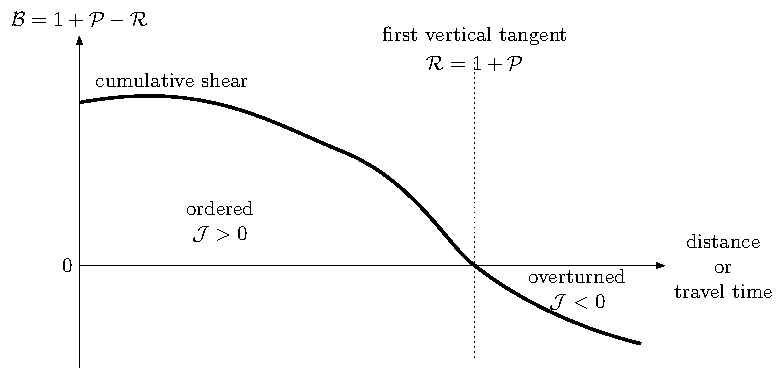
\includegraphics{../figures/Figure2.pdf}
\caption{Conceptual order budget. The sign of \(\mathcal{B}=1+\mathcal{P}-\mathcal{R}\) is the sign of the order Jacobian. Local reverse shear need not cause overturning; a vertical tangent appears only after cumulative reverse shear removes the initial depositional contribution and the accumulated normal-shear contribution.}
\label{fig:budget}
\end{figure}

\section{Stokes constraints on isochrone order}

\subsection{Exact stress decomposition of vertical shear}

The order theorem applies to any velocity field satisfying Equations~\ref{eq:incompressibility}--\ref{eq:age}. For steady, isothermal or thermomechanically prescribed, isotropic generalized-Newtonian Stokes flow, the momentum and constitutive equations constrain the vertical shear:
\begin{align}
\nabla\cdot\bm{u}&=0,
\label{eq:mass}\\
-\nabla p+\nabla\cdot\bm{\tau}+\rho\bm{g}&=\bm{0},
\label{eq:momentum}\\
\bm{\tau}&=2\eta\bm{D},
\qquad
\bm{D}=\tfrac12\left(\nabla\bm{u}+\nabla\bm{u}^{\mathsf T}\right),
\qquad \eta>0.
\label{eq:rheology}
\end{align}
Here, \(p\) is pressure, \(\rho\) is ice density, \(\bm{g}\) is gravitational acceleration, \(\bm{\tau}\) is the deviatoric stress tensor, \(\bm{D}\) is the strain-rate tensor and \(\eta\) is the positive scalar effective viscosity (constant for linear-viscous ice, or dependent on temperature and effective strain rate for Glen-law ice; positivity of \(\eta\) is required for the stress--shear sign relations below). Anisotropic rheology is discussed in the Discussion.

With \(z\) vertical and gravity having no horizontal component, the horizontal momentum equation is
\begin{equation}
-p_x+\tau_{xx,x}+\tau_{xz,z}=0.
\label{eq:xmomentum}
\end{equation}
Write
\begin{equation}
p=p_{\mathrm{atm}}+\rho g(s-z)+p_{\mathrm{nh}},
\label{eq:pressuredecomp}
\end{equation}
where \(g=|\bm{g}|\), \(p_{\mathrm{atm}}\) is atmospheric pressure and \(p_{\mathrm{nh}}\) contains all nonhydrostatic pressure, including the finite-slope surface correction. Integrating Equation~\ref{eq:xmomentum} downward from the free surface, with \(\zeta\) as the vertical coordinate of integration, gives
\begin{equation}
\tau_{xz}(x,z)
=\tau_{xz}^{s}
-\rho g s_x(s-z)
+\int_z^s\left(\tau_{xx,x}-p_{\mathrm{nh},x}\right)\,\mathop{}\!\mathrm{d}\zeta,
\label{eq:tauxzint}
\end{equation}
where the superscript \(s\) denotes evaluation at the upper surface. From Equation~\ref{eq:rheology}, the off-diagonal strain-rate component is \(D_{xz}=\tfrac12(u_z+w_x)\), so \(\tau_{xz}=2\eta D_{xz}=\eta(u_z+w_x)\), and therefore
\begin{equation}
 u_z
 =\underbrace{\frac{\rho g(s-z)(-s_x)}{\eta}}_{G}
 +\underbrace{
 \left[
 -w_x+\frac{\tau_{xz}^{s}}{\eta}
 +\frac{1}{\eta}\int_z^s
 \left(\tau_{xx,x}-p_{\mathrm{nh},x}\right)\,\mathop{}\!\mathrm{d}\zeta
 \right]}_{R_{\mathrm{S}}}.
\label{eq:uzdecomp}
\end{equation}
For a surface descending downstream (\(s_x\leq0\)), the gravity-driven term \(G\) is nonnegative and favors order preservation. The local velocity-gradient residual \(R_{\mathrm{S}}\) (units \(\mathrm{yr^{-1}}\)) collects the non-shallow Stokes contributions omitted from the shallow-ice shear balance: horizontal gradients of vertical velocity, longitudinal deviatoric stress gradients, nonhydrostatic pressure gradients and the Cartesian surface shear-stress component.

Substituting Equation~\ref{eq:uzdecomp} into Equation~\ref{eq:Jexact} gives
\begin{equation}
\mathcal{J}=\frac{u}{u_{s0}}
\left(1+\mathcal{G}+\mathcal{F}\right),
\label{eq:Jfullstokes}
\end{equation}
where \(\mathcal{G}\) and \(\mathcal{F}\) are the dimensionless trajectory-integrated contributions of \(G\) and \(R_{\mathrm{S}}\),
\begin{align}
\mathcal{G}&=\dot a_0u_{s0}
\int_{x_0}^{x}\frac{G}{u^3}\,\mathop{}\!\mathrm{d}\xi\geq0,
\label{eq:Ggrav}\\
\mathcal{F}&=\dot a_0u_{s0}
\int_{x_0}^{x}\frac{R_{\mathrm{S}}}{u^3}\,\mathop{}\!\mathrm{d}\xi.
\label{eq:Gfs}
\end{align}
The exact Stokes condition for a vertical or overturned isochrone is
\begin{equation}
\mathcal{F}\leq-\left(1+\mathcal{G}\right).
\label{eq:FSfailure}
\end{equation}
A conservative sufficient condition for no overturning is
\begin{equation}
\dot a_0u_{s0}
\int_{x_0}^{x}
\frac{\left[R_{\mathrm{S}}\right]_{-}}{u^3}\,\mathop{}\!\mathrm{d}\xi<1,
\label{eq:FSsufficient}
\end{equation}
which discards all positive contributions, including gravity-driven shear, and is therefore straightforward to bound.

\subsection{Stokes mechanics permits reverse shear}

Neither incompressibility nor the Stokes equations fixes the sign of \(u_z\). Even where \(s_x\leq0\) makes the gravity-driven term \(G\) nonnegative in Equation~\ref{eq:uzdecomp}, the residual \(R_{\mathrm{S}}\) can exceed \(G\) in magnitude and produce local reverse shear (\(u_z<0\)) whenever vertical-velocity gradients (\(-w_x\)), longitudinal stress gradients (\(\tau_{xx,x}\)) or nonhydrostatic pressure gradients (\(-p_{\mathrm{nh},x}\)) are sufficiently negative. Analytical rough-bed Stokes solutions accordingly predict local velocity maxima and minima, and hence intervals of \(u_z<0\), even for gravity-driven linear-viscous flow \citep{Gudmundsson1997linear}; the extrusion-flow literature similarly confirms that surface-fast velocity profiles are not guaranteed pointwise in Stokes flow \citep{Waddington2010}. Local reverse shear is necessary but not sufficient for overturning: order reversal further requires the integrated reverse-shear contribution \(\mathcal{R}\) to reach \(1+\mathcal{P}\).

At sufficiently steep bed relief or sharp subglacial valley corners, the one-way-flow assumption itself---namely \(u(x,z)>0\) along trajectories (Equation~\ref{eq:forwardflow}), which excludes flow reversal and closed recirculation---can fail. Steep sinusoidal beds and sharp subglacial corners can generate separated, closed recirculating eddies \citep{Gudmundsson1997nonlinear,Moffatt1964,MeyerCreyts2017}. Such closed orbits are distinct from the open-trajectory overturning analyzed here and are incompatible with a steady surface-sourced age field: integrating Equation~\ref{eq:age} around any closed streamline of period \(T>0\) would require
\begin{equation*}
\tau(T)-\tau(0)
=
\int_0^T\frac{\mathrm{D}\tau}{\mathrm{D}t}\,\mathop{}\!\mathrm{d} t
=T,
\end{equation*}
contradicting return to the same Eulerian point, where \(\tau(T)=\tau(0)\). A recirculating eddy can deform inherited layers or trap ice supplied by another boundary, whereas the overturning considered here occurs along open trajectories that exit the domain (as in the point-margin calculations below).

\section{Regimes that preserve order}

\subsection{Shallow-ice flow}

Under the conventional leading-order shallow-ice approximation (SIA), both the stress balance and the strain rate simplify: horizontal shear stress is governed by the hydrostatic driving stress,
\begin{equation}
\tau_{xz}\simeq-\rho g(s-z)s_x,
\label{eq:SIAstress}
\end{equation}
and horizontal gradients of vertical velocity are neglected relative to vertical shear (\(w_x\ll u_z\)), so the isotropic Glen-type constitutive relation reduces to \(\tau_{xz}\simeq\eta u_z\) \citep{CuffeyPaterson2010}. Together, these two SIA approximations tie the sign of \(u_z\) directly to the sign of \(-s_x\), while leading-order basal sliding adds only a depth-independent horizontal velocity. For strictly downhill, one-way flow (\(s_x<0\) and \(u>0\)), \(\tau_{xz}>0\) throughout the column and therefore
\begin{equation}
 u_z\geq0,
 \qquad \mathcal{R}=0,
 \qquad \mathcal{J}>0.
\label{eq:SIAorder}
\end{equation}
Thus steady, surface-generated stratigraphy preserves its depositional order under leading-order SIA wherever the surface slopes strictly downhill and horizontal velocity remains positive. A fixed bed obstacle can still produce arches, troughs and finite layer curvature in SIA flow, but cannot overturn an isochrone within these assumptions. This result does not extend to ice divides, stagnation points, flow reversals or segments with adverse surface slope (\(s_x>0\)), where the downhill SIA assumptions fail.

\subsection{Regular thin-film Stokes flow}

Let
\begin{equation}
\varepsilon=\frac{H}{L}\ll1
\label{eq:aspectratio}
\end{equation}
be the aspect ratio of a smooth glacier of characteristic thickness \(H\), horizontal variation scale \(L\) and characteristic horizontal speed \(U\). Higher-order thin-film models reproduce the Stokes solution to second order in \(\varepsilon\) under regular asymptotic assumptions across a range of basal slip regimes \citep{Blatter1995,SchoofHindmarsh2010}. In this regular thin-film scaling, incompressibility (\(u_x+w_z=0\)) sets the vertical velocity scale \(W=O(\varepsilon U)\), so \(w_x=O(W/L)=O(\varepsilon^2 U/H)\). With characteristic effective viscosity \(\eta_0\), the leading shear stress scales as \(\tau_{xz}=O(\eta_0 U/H)\), whereas longitudinal deviatoric stress scales as \(\tau_{xx}=2\eta u_x=O(\eta_0 U/L)=O(\varepsilon\eta_0 U/H)\). Vertical momentum balance (\(-p_{\mathrm{nh},z}+\tau_{xz,x}+\tau_{zz,z}=0\)) likewise gives \(p_{\mathrm{nh}}=O(\varepsilon\eta_0 U/H)\), so integrating \((\tau_{xx,x}-p_{\mathrm{nh},x})/\eta\) over depth \(H\) contributes \(O(\varepsilon^2 U/H)\). At the traction-free surface with slope \(s_x=O(\varepsilon)\), the Cartesian surface shear component satisfies \(\tau_{xz}^{s}=O(\varepsilon\tau_{xx}^{s})+O(\varepsilon p_{\mathrm{nh}}^{s})=O(\varepsilon^2\eta_0 U/H)\), so \(\tau_{xz}^{s}/\eta=O(\varepsilon^2 U/H)\). Every term in the local velocity-gradient residual \(R_{\mathrm{S}}\) (Equation~\ref{eq:uzdecomp}) therefore scales as
\begin{equation}
R_{\mathrm{S}}=O\!\left(\varepsilon^2\frac{U}{H}\right).
\label{eq:RFSscale}
\end{equation}

Recall that \(R_{\mathrm{S}}\) is a local velocity-gradient contribution (units \(\mathrm{yr^{-1}}\)), whereas \(\mathcal{F}\) (Equation~\ref{eq:Gfs}) is its dimensionless cumulative contribution integrated along a trajectory. Substituting Equation~\ref{eq:RFSscale} into Equation~\ref{eq:Gfs} over a trajectory segment of horizontal length \(\Delta x=O(L)=O(H/\varepsilon)\), along which \(u\) and \(u_{s0}\) remain comparable to \(U\) and \(\dot a_0=O(\dot a)\), yields
\begin{equation}
\mathcal{F}
=\dot a_0u_{s0}\int_{x_0}^{x}\frac{R_{\mathrm{S}}}{u^3}\,\mathop{}\!\mathrm{d}\xi
\sim (\dot a\,U)\,\frac{\varepsilon^2 U/H}{U^3}\,\frac{H}{\varepsilon}
=O\!\left(\frac{\dot a}{U}\varepsilon\right).
\label{eq:GFSscale}
\end{equation}
Thus small regular Stokes corrections cannot erase the unit depositional contribution when
\begin{equation}
\frac{\dot a}{U}\varepsilon\ll1.
\label{eq:thinorder}
\end{equation}
This asymptotic regime excludes divides, abrupt sliding transitions, contact zones, steep obstacles, very slow flow and other regions where the thin-film expansion is singular or nonuniform.

\subsection{A sufficient bound for a localized obstacle}

The cumulative criterion bounds the effect of a localized obstacle without requiring pointwise monotonic shear.

\medskip
\noindent\textbf{Proposition 1 (Localized reverse-shear bound).}
Suppose reverse shear is confined to a trajectory segment of horizontal length \(\ell\). On that segment, assume
\begin{equation}
 u\geq U_{\min}>0,
 \qquad
 u_{s0}\leq U_{\mathrm{dep}},
 \qquad
 u_z^-\leq \dot\gamma_{\mathrm{rev}},
\label{eq:boundassumptions}
\end{equation}
where \(U_{\min}\) is the minimum horizontal speed on the segment, \(U_{\mathrm{dep}}\) bounds the horizontal speed at deposition, and \(\dot\gamma_{\mathrm{rev}}\) bounds the reverse vertical shear rate. Then
\begin{equation}
\mathcal{R}\leq
\frac{\dot a_0U_{\mathrm{dep}}\dot\gamma_{\mathrm{rev}}\ell}
{U_{\min}^{3}}.
\label{eq:obstaclebound}
\end{equation}
A sufficient condition for no overturning is that the right-hand side be less than one.

The derivation of Equation~\ref{eq:obstaclebound} from Equation~\ref{eq:Rdef} is given in Appendix~\ref{app:proofs}.

For an isolated obstacle whose horizontal and vertical influence scales are both \(O(H)\), with non-stagnant throughflow,
\begin{equation}
\mathcal{R}=O\!\left(\frac{\dot a}{U}\right).
\label{eq:isolatedscale}
\end{equation}
In a typical interior or flank setting where \(U\gg\dot a\), an isolated fixed bump can create local extrusion and visible draping while remaining far from the reverse-shear value required for a vertical tangent. More generally, setting the right-hand side of Equation~\ref{eq:obstaclebound} equal to one and solving for length gives
\begin{equation}
\ell
\gtrsim
\frac{U_{\min}^{3}}
{\dot a_0U_{\mathrm{dep}}\dot\gamma_{\mathrm{rev}}}.
\label{eq:lengththreshold}
\end{equation}
Slow throughflow reduces this required length through the \(U_{\min}^{3}\) numerator. For scale, take \(\dot a_0=0.05~\mathrm{m\,yr^{-1}}\), \(U_{\mathrm{dep}}=10~\mathrm{m\,yr^{-1}}\), \(\dot\gamma_{\mathrm{rev}}=0.01~\mathrm{yr^{-1}}\) and \(\ell=1~\mathrm{km}\). Equation~\ref{eq:obstaclebound} gives \(\mathcal{R}\leq0.005\) when \(U_{\min}=10~\mathrm{m\,yr^{-1}}\), which rules out overturning under these assumed bounds. With \(U_{\min}=1~\mathrm{m\,yr^{-1}}\), the bound is \(\mathcal{R}\leq5\) and no longer rules it out.

For non-stagnant flow, localized deformation and a small accumulation-to-speed ratio, Equation~\ref{eq:obstaclebound} explains why flow over an isolated bump commonly preserves isochrone order.

\subsection{First-order cancellation over periodic roughness about plug flow}

Fixed periodic roughness can also have weak cumulative effect through cancellation about a plug-flow background. Let
\begin{equation}
 u(x,z;\epsilon_b)=U_b+\epsilon_b u_1(x,z)+O(\epsilon_b^2),
 \qquad U_b>0,
\label{eq:plugperturbation}
\end{equation}
where \(\epsilon_b\) is a small amplitude parameter, \(U_b>0\) is spatially uniform, \(u_1\) is periodic in \(x\), and \(k\) is its wavenumber. The perturbation has wavelength \(2\pi/k\) and zero horizontal mean at each elevation. Along the unperturbed trajectory \(z=z_0\),
\begin{equation}
\frac{u_z}{u^3}
=\epsilon_b\frac{u_{1,z}(x,z_0)}{U_b^3}+O(\epsilon_b^2).
\label{eq:periodicshear}
\end{equation}
Therefore, over one complete wavelength,
\begin{equation}
\int_{x}^{x+2\pi/k}\frac{u_z}{u^3}\,\mathop{}\!\mathrm{d}\xi=O(\epsilon_b^2).
\label{eq:periodiccancel}
\end{equation}
Appendix~\ref{app:periodic} gives the expansion leading to Equation~\ref{eq:periodiccancel}. The perturbative frictionless rough-bed solution of \citet{Gudmundsson1997linear} has this plug-flow structure: local extrusion occurs, but its first-order stoss- and lee-side contributions cancel over a complete symmetric wavelength.

The first-order cancellation in Equation~\ref{eq:periodiccancel} does not apply to a sheared background, a solitary asymmetric obstacle, a finite path ending mid-cycle, strongly nonlinear roughness or near-stagnant trajectories.

\section{Trajectory diagnostic for Stokes models}

The order criterion can be evaluated without explicitly solving the age equation or advecting a dense family of isochrones. Start trajectories in a surface accumulation zone and record \(x_0\), \(\dot a_0\) and \(u_{s0}\). With \(t\) denoting elapsed time since deposition (equal to \(\tau\) along a trajectory started at \(\tau=0\) at the surface), integrate along each trajectory
\begin{align}
\frac{\mathop{}\!\mathrm{d} x}{\mathop{}\!\mathrm{d} t}&=u,
&
\frac{\mathop{}\!\mathrm{d} z}{\mathop{}\!\mathrm{d} t}&=w,
\label{eq:trajectory}\\
\frac{\mathop{}\!\mathrm{d}\mathcal{P}}{\mathop{}\!\mathrm{d} t}
&=\dot a_0u_{s0}\frac{u_z^+}{u^2},
&
\frac{\mathop{}\!\mathrm{d}\mathcal{R}}{\mathop{}\!\mathrm{d} t}
&=\dot a_0u_{s0}\frac{u_z^-}{u^2},
\label{eq:PRode}
\end{align}
with \(\mathcal{P}(0)=\mathcal{R}(0)=0\). Then
\begin{equation}
\mathcal{J}(t)=\frac{u(t)}{u_{s0}}
\left[1+\mathcal{P}(t)-\mathcal{R}(t)\right].
\label{eq:Jdiagnostic}
\end{equation}
Equations~\ref{eq:trajectory}--\ref{eq:Jdiagnostic} give a method-of-characteristics implementation of the age transport and its order sensitivity. Equation~\ref{eq:trajectory} traces a characteristic from the deposition boundary, Equation~\ref{eq:PRode} accumulates the signed shear history that controls separation from neighboring surface origins, and Equation~\ref{eq:Jdiagnostic} gives the resulting Jacobian without finite differencing neighboring trajectories.

For prescribed material lines or geometries containing counterflow, we calculate signed local orientation directly from the deformation gradient. Let \(\bm{X}(t;\bm{X}_0)\) be the flow map and \(\bm{F}=\partial\bm{X}/\partial\bm{X}_0\). Along a steady characteristic,
\begin{equation}
\frac{\mathop{}\!\mathrm{d}\bm{X}}{\mathop{}\!\mathrm{d}t}=\bm{u}(\bm{X}),
\qquad
\frac{\mathop{}\!\mathrm{d}\bm{F}}{\mathop{}\!\mathrm{d}t}
=\nabla\bm{u}(\bm{X})\bm{F},
\qquad
\bm{F}(0)=\bm{I}.
\label{eq:deformationgradient}
\end{equation}
An initial material-line tangent \(\bm{T}_0=[1,m_0]^{\mathsf T}\) evolves as \(\bm{T}=\bm{F}\bm{T}_0\), so its signed horizontal-order metric is
\begin{equation}
\mathcal{J}_{\mathrm{T}}=T_x=F_{11}+m_0F_{12}.
\label{eq:tangentJ}
\end{equation}
For a surface-deposition characteristic, \(m_0=s_x(x_0)\) and Equation~\ref{eq:tangentJ} is the order Jacobian \(\mathcal{J}\) (Appendix~\ref{app:inverse}). For a horizontal incoming material line, \(m_0=0\) and \(\mathcal{J}_{\mathrm{T}}=F_{11}\); this is a line-orientation metric rather than the surface-deposition Jacobian unless an upstream age boundary is supplied. The time-parameterized calculation contains no division by \(u\), remains regular when \(u=0\), and does not require a time-dependent layer simulation. Below, \(J\) denotes the applicable directly integrated metric in each numerical figure.

For one-way, surface-sourced flow, the budget diagnostic is
\begin{equation}
\min_t\left[1+\mathcal{P}(t)-\mathcal{R}(t)\right]
\begin{cases}
>0, & \text{order preserved},\\
=0, & \text{first vertical tangent},\\
<0, & \text{overturned steady isochrone}.
\end{cases}
\label{eq:numericaltest}
\end{equation}

A robust implementation should include four checks. First, compare Equation~\ref{eq:Jdiagnostic} with \(-\dot a_0\tau_z\) from an independently solved steady age equation. Second, advect at least one pair of neighboring particles to verify the sign of \(\partial x/\partial x_0|_{\tau}\). Third, use Equation~\ref{eq:tangentJ} where \(u\) approaches zero or reverses, and diagnose recirculation with the full trajectory topology. Fourth, test the velocity-gradient calculation against interpolation, sampling and mesh resolution. Separate storage of \(\mathcal{P}\) and \(\mathcal{R}\) is preferable to integrating their difference because large compensating contributions can otherwise obscure numerical error.

For transient flow, Equation~\ref{eq:Jdiagnostic} is not valid because the steady travel-time representation fails. The time-dependent analogue of Equation~\ref{eq:deformationgradient}, with \(\bm{u}=\bm{u}(\bm{X},t)\), remains valid, but the calculation must also retain deposition time in the two-parameter source map. The steady order budget remains useful as a baseline and as a diagnostic applied to quasi-steady snapshots.

\section{Stokes numerical experiments}

I present two numerical examples that evaluate the direct tangent-order metric in contrasting steady Stokes configurations: a finite convergent point-margin flow and a periodic sinusoidal-bed sweep. Both examples solve steady, incompressible Stokes flow with \(\rho=917~\mathrm{kg\,m^{-3}}\), a traction-free upper surface and an impermeable bed obeying
\begin{equation}
u_t=C\tau_b,
\qquad
u_n=0,
\qquad
\tau_b=-\bm{t}\mathbin{\cdot}\bm{\sigma}\mathbin{\cdot}\bm{n},
\label{eq:linearsliding}
\end{equation}
where \(C=10^{-5}~\mathrm{m\,yr^{-1}\,Pa^{-1}}\) (so \(\beta=C^{-1}=10^5~\mathrm{Pa\,yr\,m^{-1}}\) and \(\tau_b u_t=C\tau_b^2\geq0\)). Each configuration is solved first for linear-viscous ice with constant viscosity \(\eta=2.5\times10^8~\mathrm{Pa\,yr}\) and then for isotropic nonlinear Glen ice with stress exponent \(n=3\) and effective viscosity
\begin{equation}
\eta(\bm{D})=\tfrac12 A_{\mathrm{G}}^{-1/n}\left(D_e^2+D_0^2\right)^{(1-n)/(2n)},
\qquad
D_e=\sqrt{\tfrac12\bm{D}:\bm{D}},
\label{eq:glenrheology}
\end{equation}
using cold-ice fluidity \(A_{\mathrm{G}}=6.8\times10^{-26}~\mathrm{Pa^{-3}\,s^{-1}}=2.15\times10^{-18}~\mathrm{Pa^{-3}\,yr^{-1}}\) at \(-25^{\circ}\mathrm{C}\) \citep{CuffeyPaterson2010} and strain-rate regularization \(D_0=10^{-10}~\mathrm{yr^{-1}}\). The Stokes equations are discretized with Taylor--Hood elements, imposing basal impermeability with symmetric Nitsche terms, and the variational equation (Equations~\ref{eq:deformationgradient}--\ref{eq:tangentJ}) is integrated along characteristics of the computed velocity. I evaluate \(\mathcal{J}_{\mathrm{T}}=T_x\) uniformly across both examples because it remains regular through counterflow and near stagnation in the point-margin flow (where the \(u^{-3}\) integrals \(\mathcal{P}\) and \(\mathcal{R}\) become singular) while coinciding identically with \(\mathcal{J}=(u/u_{s0})(1+\mathcal{P}-\mathcal{R})\) along one-way surface-sourced trajectories in the periodic sinusoidal-bed sweep.

\subsection{Finite convergent point-margin flow}

The first experiment is a deliberately idealized analogue motivated by broad features near the Allan Hills nunatak. The modeled bed has an exposed-rock point margin, strong thickening from left to right and opposing shallow flows so that the boundary-value mechanism can be tested without relying on the exact geometry of one place. The domain is \(2~\mathrm{km}\) long, and thickness increases smoothly from zero at the left point margin to \(360~\mathrm{m}\) at the right boundary. Surface slope changes from \(-0.035\) on the thin side to \(0.012\) on the thick side, producing rightward flow near the margin and leftward inflow from the thick side. Bed and surface meet at one point, so there is no left boundary facet or left flux. At the right boundary, \(u(z)\) is the corresponding SIA-plus-sliding velocity profile---quadratic in height above the bed for linear-viscous ice and quartic for \(n=3\) Glen ice---scaled to one percent of the reference SIA flux, with \(w=0\); at \(-25^{\circ}\mathrm{C}\) the two rheologies carry nearly identical inward fluxes (\(1.47\) and \(1.46~\mathrm{m^2\,yr^{-1}}\)). The surface remains traction free; its steady mass balance is therefore diagnosed from the computed normal velocity rather than prescribed.

Figure~\ref{fig:nunatak-margin} summarizes the linear-viscous experiment: panel (a) gives the geometry and boundary conditions, panels (b--c) show horizontal flow, selected paths and vertical velocity, and panel (d) maps minimum \(J\) over inlet height and slope. Panel (e) follows one initially horizontal near-bed line, while panel (f) resolves the S-shaped fold in which a negative-\(J\) interval migrates, so local segments pass from ordered to unordered and back to ordered. Horizontal incoming lines reach a minimum sampled value of \(J=-0.1936\); restricting the inlet source height to \(\sigma_0\geq0.05\) still gives \(J=-0.0574\). The plotted line begins at \(\sigma_0=0.049\); its endpoint first reaches \(J=0\) after \(130.2~\mathrm{kyr}\) and reaches \(J=-0.072\) after \(136.2~\mathrm{kyr}\). The point-margin value changes from \(-0.1946\) to \(-0.1934\) across the three meshes, and positive-thickness truncations converge toward the same result (Figure~\ref{fig:nunatak-convergence}). A control imposing uniform surface ablation on the same geometry remains ordered, with \(J_{\min}=0.3075\); the reversal therefore depends on the surface-flux closure as well as geometry.

\begin{figure}[t]
\centering
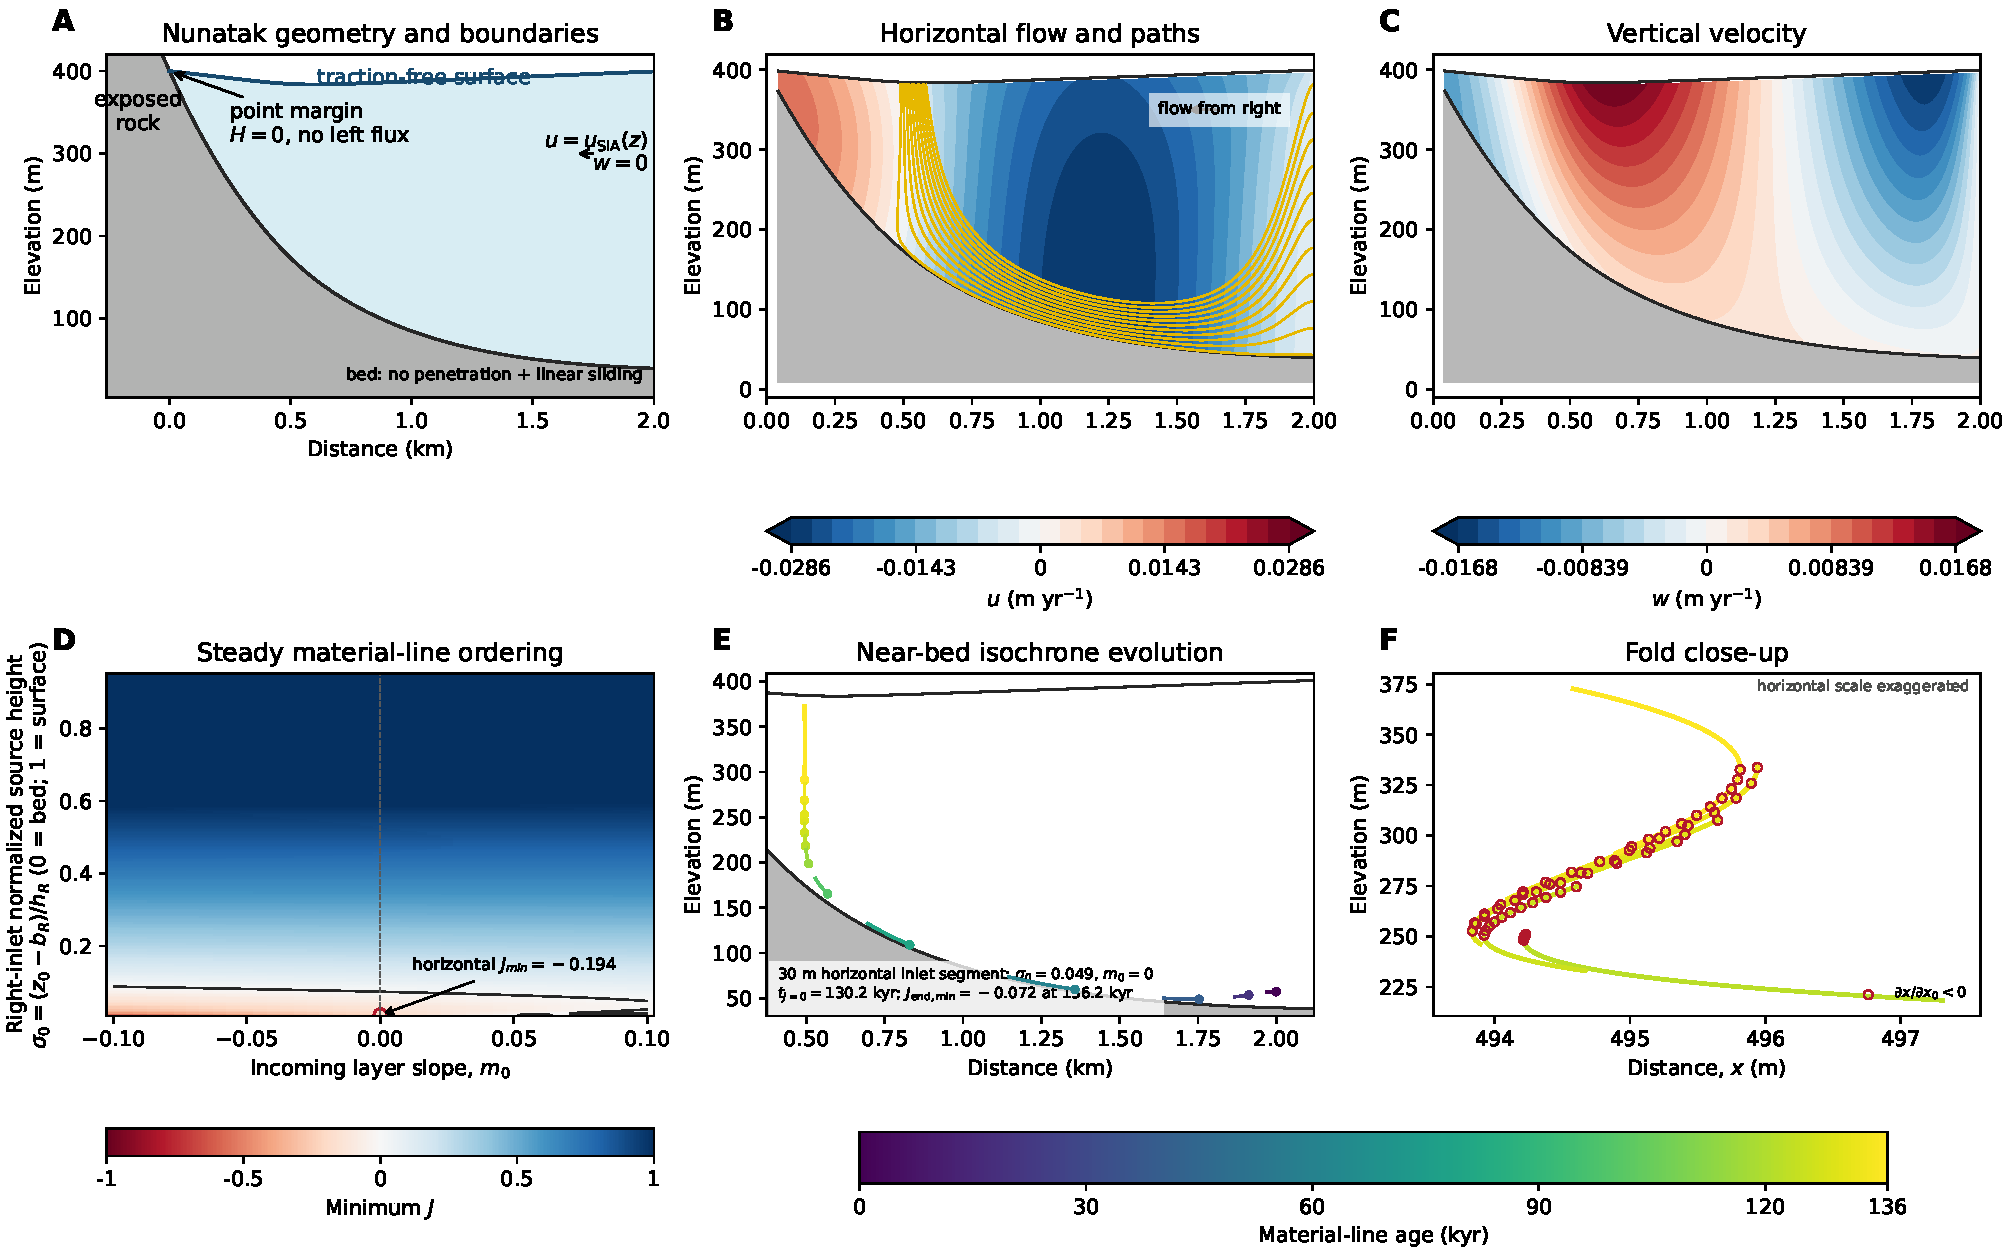
\includegraphics[width=\textwidth]{../figures/allan_hills_nunatak_margin.pdf}
\caption{Steady reversal of an incoming material line in a finite convergent point-margin flow with linear-viscous rheology (\(\eta=2.5\times10^8~\mathrm{Pa\,yr}\)). (a) Geometry and boundary conditions. The right boundary has the plotted linear-viscous SIA-shaped horizontal inflow and \(w=0\); bed and surface meet at the left point margin. (b--c) Horizontal velocity with selected paths and vertical velocity. (d) Minimum tangent-order metric \(J=T_x\) over right-inlet source height \(\sigma_0=(z_0-b_R)/h_R\) and incoming slope \(m_0\). (e) Evolution of a \(30~\mathrm{m}\) horizontal material segment initialized with a common age near the right inlet; color gives elapsed time. (f) Fold close-up. The negative-\(J\) interval migrates along the vertically extended S-shaped line, leaving locally reordered segments behind; colored symbols mark \(J<0\) at successive elapsed times. This imposed inlet stratigraphy is not generated from surface deposition within the model domain. The fixed, traction-free geometry diagnoses the surface mass balance required for steady closure.}
\label{fig:nunatak-margin}
\end{figure}

Figure~\ref{fig:nunatak-margin-glen} shows the corresponding calculation for nonlinear Glen rheology (\(n=3\)). Strain-rate softening concentrates shear closer to the bed while stiffening the low-stress interior where the opposing flows converge, strengthening the overturning of near-bed incoming layers without introducing closed recirculation. Horizontal incoming lines reach \(J=-0.2916\) on the production mesh (25 of 193 sampled inlet heights overturn, compared with 14 for linear-viscous ice), and restricting source heights to \(\sigma_0\geq0.05\) gives \(J=-0.1728\). Along the \(30~\mathrm{m}\) horizontal segment initialized at \(\sigma_0=0.049\), the endpoint crosses \(J=0\) after \(146.3~\mathrm{kyr}\) and reaches \(J=-0.186\) after \(154.5~\mathrm{kyr}\) (Figure~\ref{fig:nunatak-margin-glen}e--f). Across the \(30\), \(20\) and \(13~\mathrm{m}\) meshes, the exact point-margin minimum varies only from \(-0.2928\) to \(-0.2913\), and positive-thickness left truncations converge monotonically from \(-0.0897\) at \(20~\mathrm{m}\) to \(-0.2899\) at \(2.5~\mathrm{m}\) (Figure~\ref{fig:nunatak-convergence-glen}). Imposing uniform steady surface ablation on the same geometry again restores positive order (\(J_{\min}=0.3071\)), confirming that the boundary mass-flux closure governs reversal under both rheologies.

\begin{figure}[t]
\centering
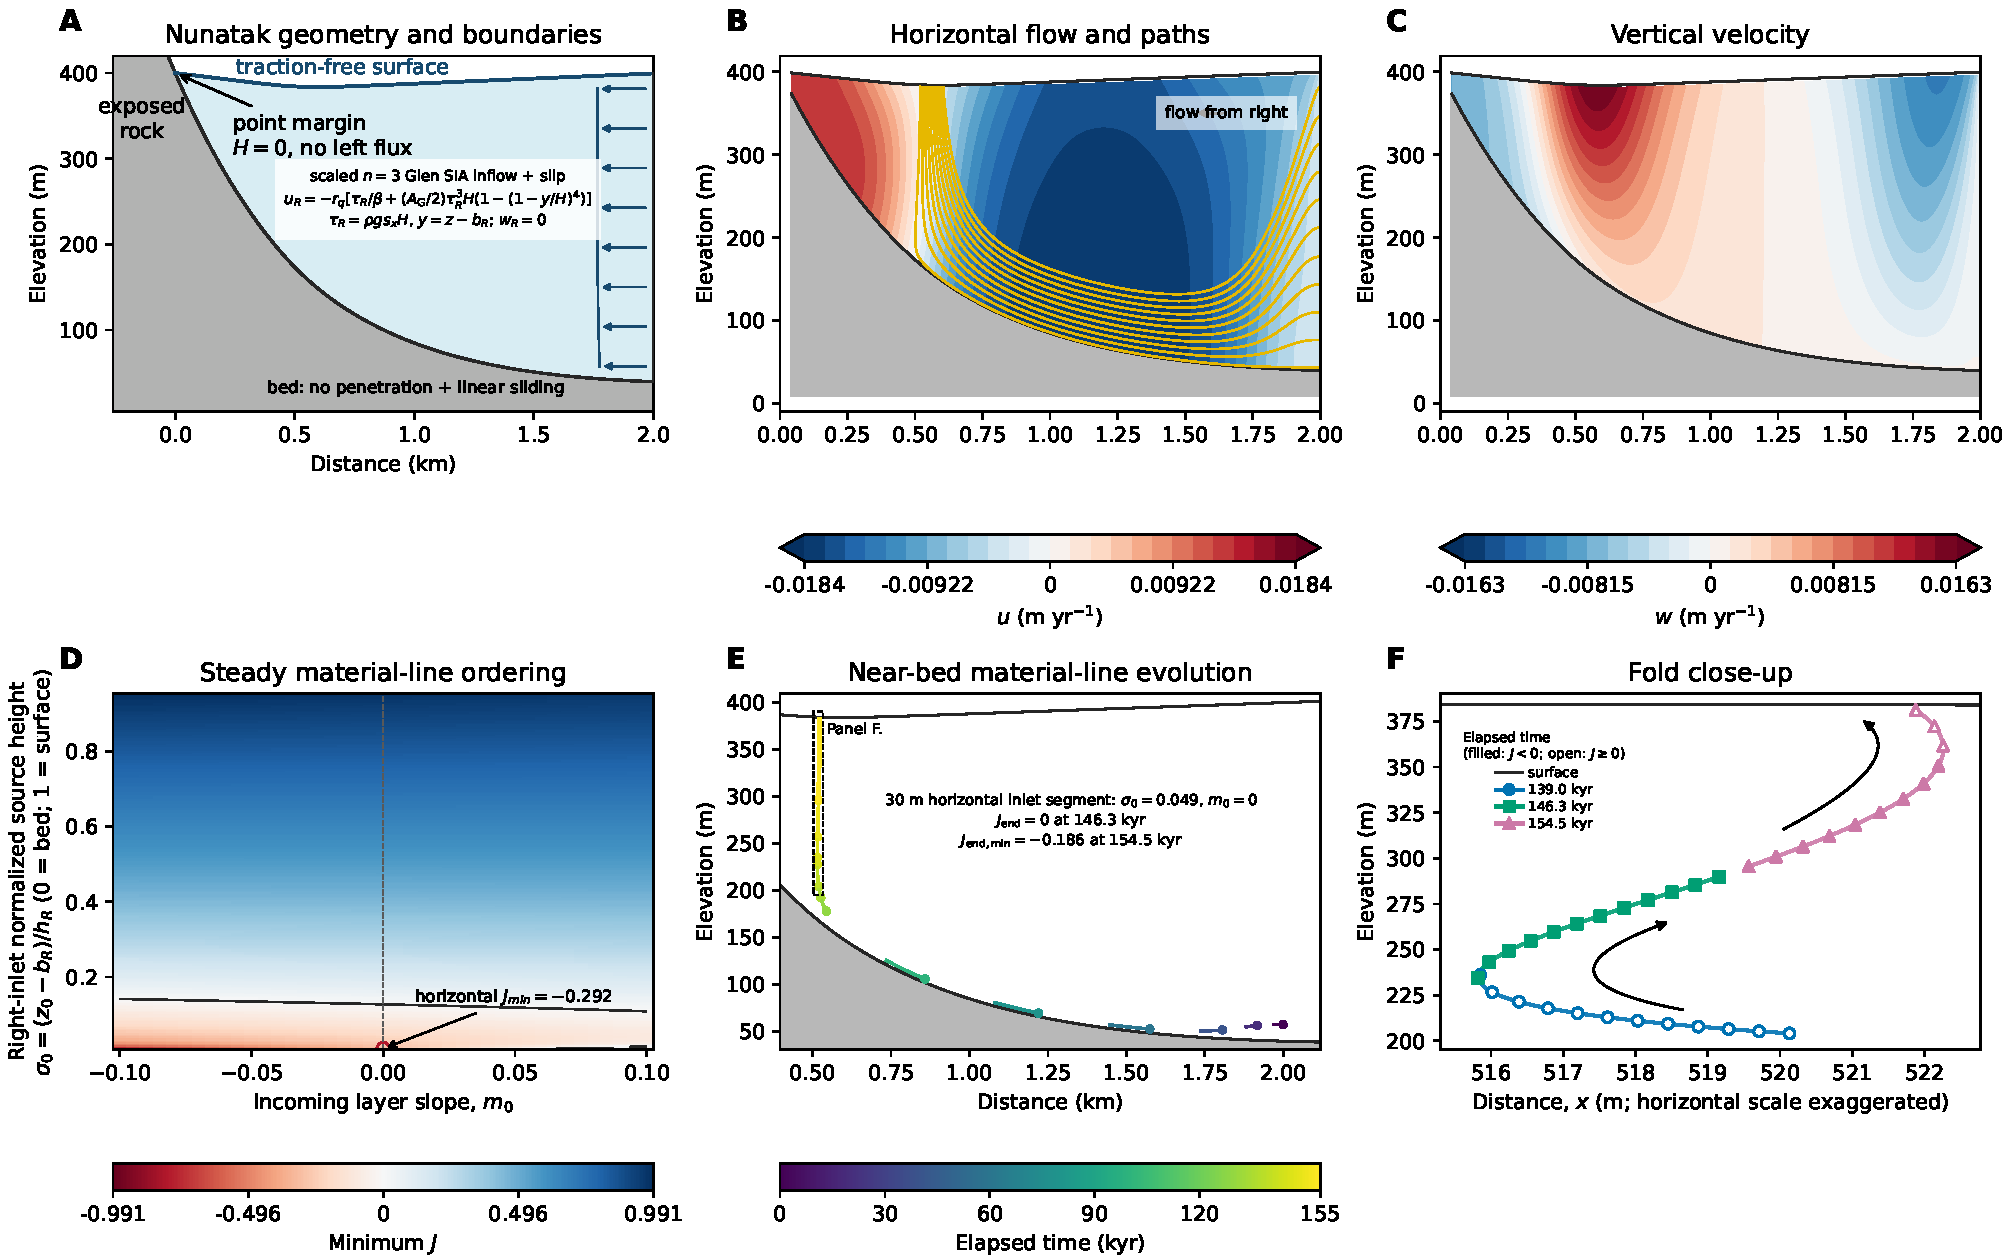
\includegraphics[width=\textwidth]{../figures/allan_hills_nunatak_margin_glen.pdf}
\caption{Steady reversal of an incoming material line in the finite convergent point-margin flow with isotropic nonlinear Glen rheology (\(n=3\), \(A_{\mathrm{G}}=6.8\times10^{-26}~\mathrm{Pa^{-3}\,s^{-1}}\)). Panels (a--f) follow the same layout and diagnostics as Figure~\ref{fig:nunatak-margin}, with the right boundary imposing the corresponding \(n=3\) SIA-plus-sliding inflow profile at one percent of the reference SIA flux. Horizontal incoming lines reach \(J_{\min}=-0.2916\), and the \(30~\mathrm{m}\) horizontal segment at \(\sigma_0=0.049\) crosses \(J=0\) at \(146.3~\mathrm{kyr}\) and reaches \(J=-0.186\) at \(154.5~\mathrm{kyr}\).}
\label{fig:nunatak-margin-glen}
\end{figure}

\subsection{Periodic sinusoidal-bed control}

The second experiment tests whether order reversal is generic to smooth bed roughness. One periodic cell has a flat surface and bed \(b(x)=-H+A\cos(2\pi x/\lambda)\); lateral boundaries are exactly periodic. Gravity is inclined at \(0.05~\mathrm{rad}\), and the surface mass balance \(\dot a=-w\) is diagnosed. Characteristics start on every accumulating surface interval, with the central \(80\%\) of its positive flux retained. Their initial tangent is horizontal, so \(J=T_x\).

Figure~\ref{fig:sinusoidal-control} summarizes the linear-viscous sweep: panel (a) defines the one-wavelength geometry, and panels (b--f) map minimum \(J\) over amplitude and wavelength for \(H=50\), 100, 160, 240 and \(320~\mathrm{m}\). The sweep spans \(A/H=0\)--0.85 and \(\lambda/H=1/12\)--12, with sliding-thickness ratio \(\beta H/\eta=0.020\)--0.128. All 750 resolved numerical cases and 80 analytical flat-bed limits preserve order. The smallest resolved value is \(J=0.6428\) at \(H=50~\mathrm{m}\), \(A/H=0.85\) and \(\lambda/H=3\); the raw minimum through surface exit is 0.4428. Another 210 short-wave cells fall below the numerical surface-signal threshold and remain unclassified. Distortion is strongest at intermediate wavelength and weakens toward the resolved short- and long-wave limits.

\begin{figure}[t]
\centering
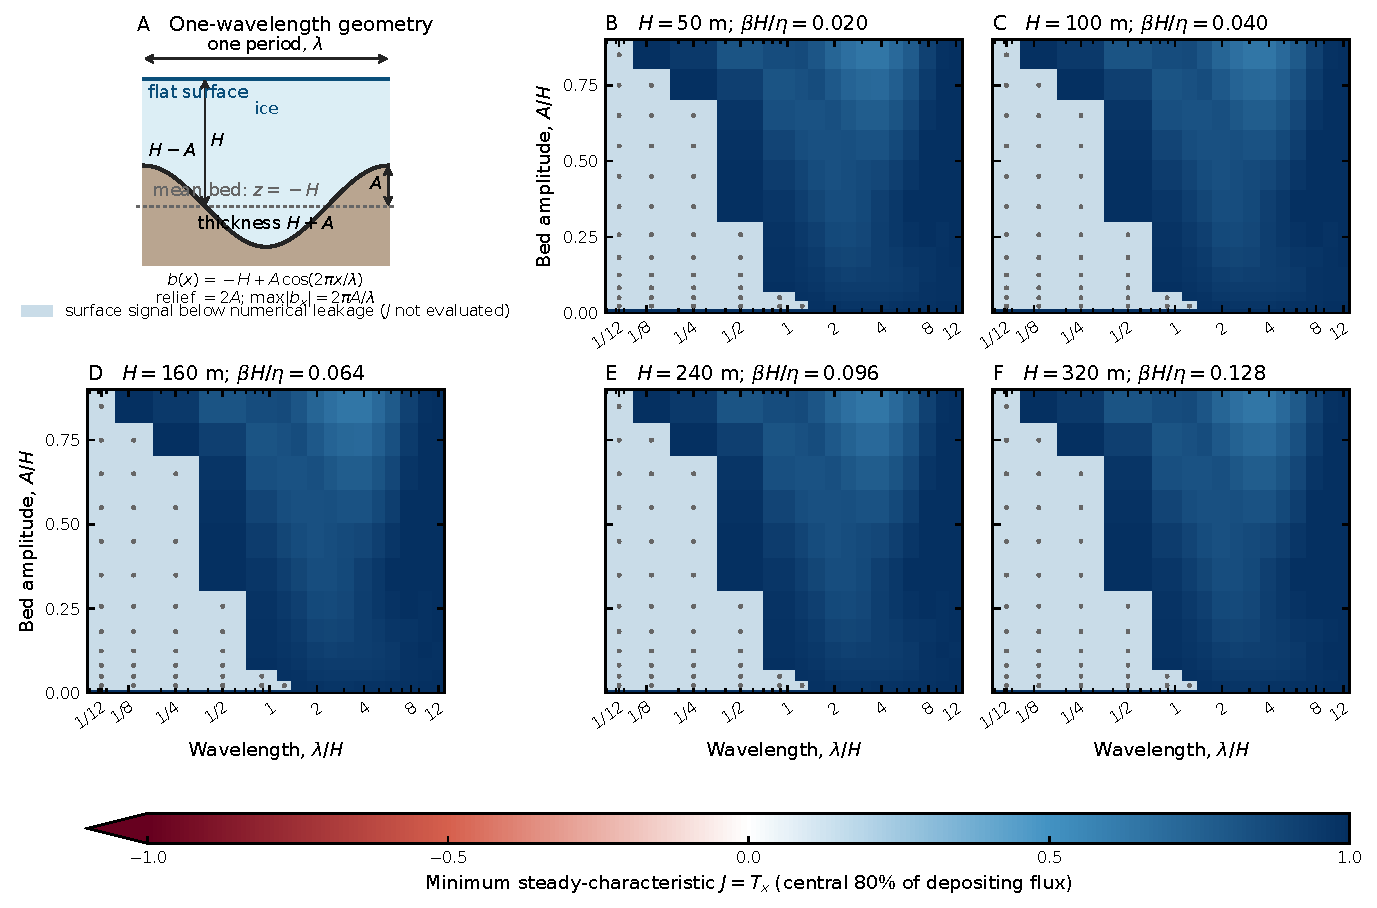
\includegraphics[width=\textwidth]{../figures/steady_characteristic_sinusoidal_parameter_map.pdf}
\caption{Steady isochrone order over sinusoidal beds for linear-viscous rheology (\(\eta=2.5\times10^8~\mathrm{Pa\,yr}\)). (a) One periodic model cell with a flat surface and bed \(b(x)=-H+A\cos(2\pi x/\lambda)\). (b--f) Minimum order metric \(J=T_x\) for five mean thicknesses; \(\beta=C^{-1}\) and \(\beta H/\eta\) is the sliding-thickness ratio. Characteristics start on the physical surface wherever the diagnosed accumulation \(\dot a=-w\) is positive, retaining the central \(80\%\) of its flux. The primary diagnostic excludes only the upper \(5\%\) of local thickness beneath surface ablation. All 750 resolved numerical cells remain ordered, with \(J_{\min}=0.6428\); 80 flat-bed cells use the analytical limit \(J=1\). Dotted pale cells mark 210 cases whose surface signal is less than ten times the RMS basal normal leakage and are not evaluated. The dotted boundary marks numerical reach, not a physical transition.}
\label{fig:sinusoidal-control}
\end{figure}

Figure~\ref{fig:sinusoidal-control-glen} repeats the sweep for nonlinear Glen rheology (\(n=3\)). Measuring internal shear with the driving-stress viscosity scale \(\eta_{\mathrm{G}}=\bigl(2A_{\mathrm{G}}\tau_{\mathrm{d}}^2\bigr)^{-1}\), where \(\tau_{\mathrm{d}}=\rho g H\sin(0.05~\mathrm{rad})\), gives \(\beta H/\eta_{\mathrm{G}}=0.011\), \(0.087\), \(0.355\), \(1.20\) and \(2.84\) across \(H=50\)--\(320~\mathrm{m}\), spanning the transition from sliding-dominated to internal-shear-dominated flow. All 745 resolved numerical cases and 80 analytical flat-bed limits again preserve order, while 215 short-wave cells fall below the surface-signal threshold. Shear-thinning over the bed crests deepens the intermediate-wavelength distortion trough relative to linear-viscous ice, lowering the smallest resolved value to \(J=0.3686\) at \(H=50~\mathrm{m}\), \(A/H=0.85\) and \(\lambda/H=4\), with a raw minimum of \(0.2562\) through surface exit; at larger \(H\), stronger surface-fast shear raises the minimum slightly to \(0.3982\) at \(320~\mathrm{m}\). Small Eulerian counterflow pockets form in deep short-wavelength troughs in 156 resolved cases, as in 160 linear-viscous cases, yet no retained surface-deposition trajectory reverses horizontal direction. Thus finite-amplitude symmetric roughness strongly compresses a surface-deposition map under both rheologies without overturning it over the resolved parameter range.

\begin{figure}[t]
\centering
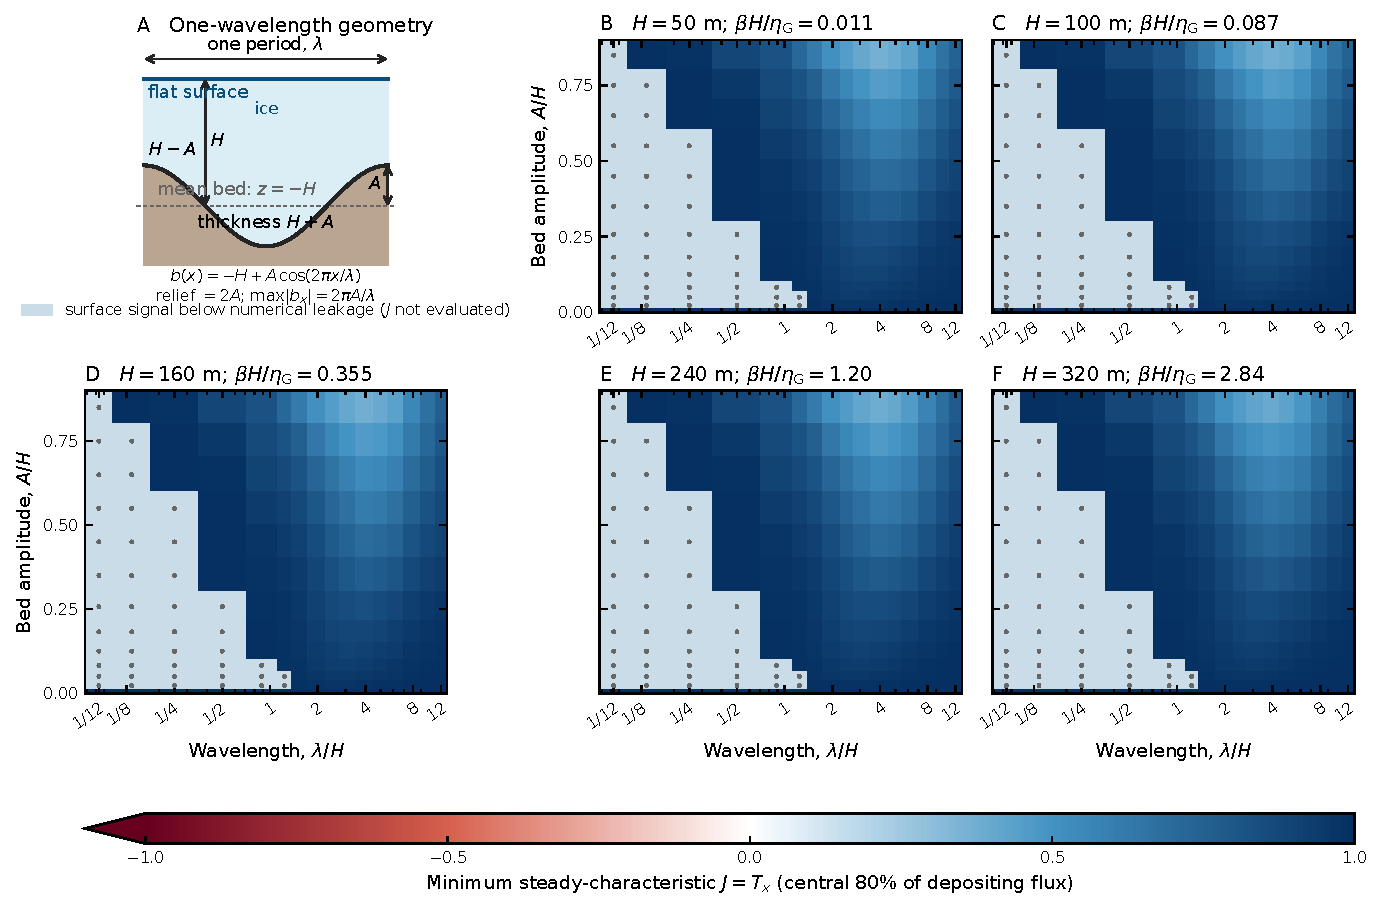
\includegraphics[width=\textwidth]{../figures/steady_characteristic_sinusoidal_glen_parameter_map.pdf}
\caption{Steady isochrone order over sinusoidal beds for isotropic nonlinear Glen rheology (\(n=3\), \(A_{\mathrm{G}}=6.8\times10^{-26}~\mathrm{Pa^{-3}\,s^{-1}}\)). Panels (a--f), source conventions and leakage screening match Figure~\ref{fig:sinusoidal-control}, with \(\eta_{\mathrm{G}}=\bigl(2A_{\mathrm{G}}\tau_{\mathrm{d}}^2\bigr)^{-1}\) denoting the characteristic Glen viscosity at mean driving stress \(\tau_{\mathrm{d}}=\rho g H\sin(0.05~\mathrm{rad})\). Across \(\beta H/\eta_{\mathrm{G}}=0.011\)--\(2.84\), all 745 resolved numerical cells remain ordered, with \(J_{\min}=0.3686\) at \(H=50~\mathrm{m}\), \(A/H=0.85\) and \(\lambda/H=4\); 80 flat-bed cells satisfy \(J=1\), and 215 dotted pale cells fall below the tenfold surface-signal-to-leakage threshold.}
\label{fig:sinusoidal-control-glen}
\end{figure}

\section{Discussion}

\subsection{Limits of the steady coordinate construction}

For flow satisfying Equations~\ref{eq:incompressibility}--\ref{eq:age}, cumulative reverse shear can overturn an isochrone when Equation~\ref{eq:verticalcondition} is met, without a change in boundary conditions. The extrusion-flow literature describes local reverse shear without evaluating this cumulative threshold. Variable density requires the mass-flux extension given in Appendix~\ref{app:density}.

Stagnation and recirculation instead violate the coordinate construction. If \(u\) vanishes or reverses, downstream position no longer parameterizes a trajectory and the \(1/u\) and \(1/u^3\) integrals become singular. Time integration via the deformation gradient (Equation~\ref{eq:deformationgradient}) remains possible, but a closed streamline cannot have the unique surface origin assumed here. The Allan Hills model of \citet{Manos2026} approaches this limit: its near-stagnant basal flow remains nonzero, yet makes the order integral sensitive to small velocities.

Material sources also restrict the theorem. Accumulation need occur only over the originating portion of the surface: a trajectory may enter through an accumulation zone (\(\dot a>0\)) and subsequently leave through a surface ablation zone (\(\dot a<0\)) or basal melting, as occurs in blue-ice areas and in our periodic sinusoidal-bed experiment. Ablation and basal melting simply truncate the trajectory at exit, whereas its deposition coordinate remains defined on the originating accumulation zone. Multiple disconnected surface sources or basal freeze-on instead require a more general label, and freeze-on can add debris-bearing structures that are not surface-deposited isochrones \citep{LeysingerVieli2018,Holschuh2026}.

Changes in geometry or basal traction leave an inherited age field that differs from the steady age solution. Divide migration, traveling traction anomalies and former ice-stream configurations can therefore seed folds later amplified by shear \citep{JacobelBindschadler1993,JacobsonWaddington2005,Wolovick2014,WolovickCreyts2016,Franke2022,Jansen2024}. These mechanisms remain distinct from overturning generated continuously in a fixed velocity field.

Finally, Equation~\ref{eq:uzdecomp} assumes isotropic scalar viscosity and the order theorem is two-dimensional. Fabric, rheological heterogeneity and non-Newtonian normal-stress differences can actively generate folds or secondary spiral flows \citep{Alley1997,ThorsteinssonWaddington2002,SchoofClarke2008,Bons2016,Bons2025}, and convergent anisotropic flow occurs in both radar observations and models \citep{Ross2020,MartinGudmundssonPritchardGagliardini2009}. In three dimensions, the relevant quantity is the two-dimensional Jacobian mapping a surface deposition patch to an equal-age surface. The scalar \(\mathcal{J}\) applies only within a coherent flow tube with negligible cross-flow.

\subsection{Implications for old-ice sites}

Allan Hills approaches several limits of the two-dimensional calculation. Ice rises into an ablation zone above steep nunatak topography \citep{Spaulding2012,Kehrl2018,Stoll2026}. \citet{Manos2026} predict nearly stagnant basal ice upstream of the nunatak: the bottom \(20~\mathrm{m}\) averages \(0.4\)--\(0.5~\mathrm{mm\,yr^{-1}}\), with local speeds of order micrometres per year, compared with \(46\)--\(49~\mathrm{mm\,yr^{-1}}\) in the Cul-de-sac. Such small \(u\) makes the \(u^{-3}\) order integral numerically sensitive. The modeled flow is also three-dimensional, with bridging stresses represented in two dimensions by the \(-w_x\) term in Equation~\ref{eq:uzdecomp}.

The point-margin experiment represents the observed thick-ice-to-thin-ice convergence and shows that this boundary-value flow can reverse an imposed incoming material line. Because layers are prescribed at the inflow boundary rather than deposited at the surface, the calculation does not test surface-sourced stratigraphy or predict overturning at Allan Hills. A site calculation would require a three-dimensional, multi-source material map built from measured geometry, basal traction and surface mass balance. Such a calculation would launch characteristics from each candidate accumulation source, follow them to the core or radar transect and evolve the two-dimensional Jacobian of the source patch. Equations~\ref{eq:deformationgradient}--\ref{eq:tangentJ} give the corresponding local calculation.

At Little Dome C, radar and flow modelling indicate strong basal thinning and possibly stagnant or disturbed ice \citep{Lilien2021,Chung2025BeyondEPICA}. Evaluating \(\mathcal{J}\) along trajectories would test whether steady flow preserves order above this basal unit.

The equations suggest four tests of an observed fold or age reversal.

\begin{enumerate}[leftmargin=*,label=(\arabic*)]
  \item \textbf{Steady geometry.} Evaluate \(\mathcal{P}\), \(\mathcal{R}\) and \(\mathcal{J}\) along source-to-core trajectories. A positive budget excludes steady overturning.
  \item \textbf{Flow topology and sources.} Test for stagnation, recirculation, freeze-on and multiple surface origins; these require the full material map.
  \item \textbf{Unsteady inheritance.} If steady flow preserves order, evaluate past changes in geometry, ablation and basal traction.
  \item \textbf{Active deformation.} If passive models underpredict folding, couple fabric and rheological heterogeneity to flow.
\end{enumerate}

In regular, shallow, non-stagnant flow, Equation~\ref{eq:obstaclebound} favors a time-dependent or rheological mechanism. In more general Stokes flow, the order criterion diagnoses overturning only if cumulative reverse shear crosses the threshold.

\section{Conclusions}

The signed order Jacobian measures depositional order in a steady two-dimensional isochrone (Equation~\ref{eq:Jexact}). It is observable as \(-\dot a_0\tau_z\) (Equation~\ref{eq:Jage}) and, while positive, is the reciprocal of the established vertical thinning function (Equation~\ref{eq:thinningrelation}). The order budget separates the initial and normal-shear contributions from cumulative reverse shear; overturning begins when \(\mathcal{R}=1+\mathcal{P}\) (Equation~\ref{eq:verticalcondition}).

Stokes mechanics permits reverse shear through longitudinal stress, nonhydrostatic pressure and horizontal gradients of vertical velocity (cf. Equation~\ref{eq:uzdecomp}). Leading-order shallow-ice flow with a strictly downhill surface slope preserves order (Equation~\ref{eq:SIAorder}), while localized obstacles and small-amplitude periodic roughness preserve it under the bounds in Equations~\ref{eq:obstaclebound} and \ref{eq:periodiccancel}. Stagnation and recirculation invalidate the one-way coordinate construction.

For both linear-viscous and nonlinear Glen (\(n=3\)) rheologies, the finite point-margin experiment folds an ordered incoming material line (Figures~\ref{fig:nunatak-margin} and \ref{fig:nunatak-margin-glen}), while the periodic sinusoidal-bed surface-deposition map remains ordered (Figures~\ref{fig:sinusoidal-control} and \ref{fig:sinusoidal-control-glen}). Both experiments use the same linear sliding law, but their source and boundary closures differ. Together they show that layer reversal is configuration dependent rather than a generic consequence of bed roughness.

The order budget at old ice sites provides a common test of whether local flow preserves deposition order. Applying it requires reconstructed trajectories and, where cross-flow or multiple source regions are important, a three-dimensional material map. An overturned isochrone complicates a climate archive, but it also preserves a mechanical record of the flow that brought ancient ice within reach.

\section*{Data availability statement}
No new observational data are presented. The published age--depth data in Figure~\ref{fig:allan-hills-context} are from the source data of \citet{Shackleton2025} and \citet{MarksPeterson2026}; the map uses Copernicus Sentinel-2 L2A imagery. The analytical results are fully specified by the equations in this manuscript. Executed notebooks and figure scripts contain the Stokes solves, trajectory calculations, numerical checks and figure generation and are available at \texttt{github.com/bradlipovsky/allan-hills-stratigraphy}.

\section*{Author contributions}
Bradley Paul Lipovsky developed the analysis and wrote the manuscript draft.

\section*{Competing interests}
None.

\section*{Acknowledgements}
The author received no funding from The Center for Old Ice Exploration (COLDEX), an NSF Science and Technology Center (NSF-2019719), for this work. The author nevertheless benefited from the Center's generous intellectual environment and is grateful for conversations with colleagues across its community.

Large-language-model coding and writing tools---OpenAI Codex (GPT-5 and \texttt{5.6-sol}, \texttt{openai.com/codex}) during initial manuscript development (3 August--1 September 2026) and peer-review revisions (October--November 2026), together with Google Antigravity (Gemini 4 Carbon) during final peer-review revisions (November 2026)---assisted with literature searches, drafting and editing prose, LaTeX formatting, numerical-code implementation and exploratory parameter sweeps. The author conceived the research question, established the physical assumptions and theoretical framing, directed all analyses, independently verified all cited sources, derivations, code and numerical results, revised all AI-assisted text and takes full responsibility for the manuscript.

\bibliographystyle{igs}
\bibliography{references}

\setcounter{secnumdepth}{1}
\appendix
\makeatletter
\@addtoreset{equation}{section}
\makeatother

\section{Notation}
\label{app:notation}

\begingroup
\small
\begin{longtable}{@{}p{0.18\textwidth}p{0.59\textwidth}p{0.17\textwidth}@{}}
\caption{Notation. Units are given for dimensional quantities used in the numerical experiments; all fluxes are ice-equivalent.}
\label{tab:notation}\\
\toprule
Symbol & Definition & Units \\
\midrule
\endfirsthead
\multicolumn{3}{@{}l}{\textit{Table~\ref{tab:notation} continued}}\\
\toprule
Symbol & Definition & Units \\
\midrule
\endhead
\bottomrule
\endfoot
\multicolumn{3}{@{}l}{\textit{Coordinates and kinematics}}\\
\(x,z\) & Horizontal and vertical Cartesian coordinates; \(x\) increases downstream. & \(\mathrm{m}\) \\
\(x_0\) & Horizontal coordinate of surface deposition; a material-origin label. & \(\mathrm{m}\) \\
\(\xi,\zeta\) & Horizontal and vertical coordinates of integration. & \(\mathrm{m}\) \\
\(z_0\) & Elevation of an unperturbed streamline (periodic calculation) or right-inlet source point (point-margin experiment). & \(\mathrm{m}\) \\
\(s(x),b(x)\) & Free-surface and bed elevations. & \(\mathrm{m}\) \\
\(H,L,\ell\) & Ice thickness, horizontal forcing scale and length of a reverse-shear segment. & \(\mathrm{m}\) \\
\(t,\tau,T\) & Time since deposition, stratigraphic age and trajectory duration or orbit period. & \(\mathrm{yr}\) \\
\(\bm{u}=[u,w]^{\mathsf T}\) & Velocity vector and its horizontal and vertical components. & \(\mathrm{m\,yr^{-1}}\) \\
\(\bm{X},\bm{X}_0\) & Current and initial material positions in the flow map. & \(\mathrm{m}\) \\
\(\bm{F},\bm{T},m_0\) & Deformation gradient, material-line tangent and its initial slope. & \(1\) \\
\(u_s,u_{s0}\) & Horizontal surface speed and its value at deposition. & \(\mathrm{m\,yr^{-1}}\) \\
\(U,W,U_b\) & Characteristic horizontal and vertical speeds and uniform background plug-flow speed. & \(\mathrm{m\,yr^{-1}}\) \\
\(U_{\min},U_{\mathrm{dep}}\) & Lower speed bound on a trajectory segment and upper bound on speed at deposition. & \(\mathrm{m\,yr^{-1}}\) \\
\(u_1\) & First-order horizontal-velocity perturbation. & \(\mathrm{m\,yr^{-1}}\) \\
\(\dot a,\dot a_0\) & Ice-equivalent surface mass-balance rate and its value at \(x_0\). & \(\mathrm{m\,yr^{-1}}\) \\
\(\psi,\Psi\) & Streamfunction per unit width and its restriction to the surface, \(\Psi(x)=\psi[x,s(x)]\). & \(\mathrm{m^2\,yr^{-1}}\) \\
\(\delta x,\delta x_0\) & Horizontal separations at observation and deposition. & \(\mathrm{m}\) \\
\multicolumn{3}{@{}l}{\textit{Parrenin--Hindmarsh coordinates (Appendix~\ref{app:parrenin})}}\\
\(Q,Q^{\mathrm{ref}}\) & Total horizontal flow-tube flux and its value at a reference position. & \(\mathrm{m^3\,yr^{-1}}\) \\
\(\Omega\) & Streamfunction normalized by total flux. & \(1\) \\
\(\pi,\theta\) & Logarithmic flux coordinates: \(\pi=\ln[Q(x)/Q^{\mathrm{ref}}]\) and \(\theta=\ln\Omega\). & \(1\) \\
\(\pi_0\) & Logarithmic flux coordinate of surface deposition. & \(1\) \\
\(\delta\pi,\delta\pi_0\) & Neighboring-particle separations in logarithmic flux at observation and deposition. & \(1\) \\
\(\alpha\) & Path-sign parameter defined by \(\delta\pi=(1-\alpha)\delta\pi_0\). & \(1\) \\
\multicolumn{3}{@{}l}{\textit{Stratigraphic order}}\\
\(\mathcal{J}\) & Isochrone-order Jacobian, \(\left.\partial x/\partial x_0\right|_\tau\). & \(1\) \\
\(\mathcal{J}_{\mathrm{T}}\) & Direct tangent-order metric, \(T_x=F_{11}+m_0F_{12}\). & \(1\) \\
\(\sigma_0\) & Normalized source height at the right inlet. & \(1\) \\
\(\lambda_z\) & Vertical thinning function for ordered stratigraphy. & \(1\) \\
\(u_z,u_z^+,u_z^-\) & Vertical shear and its positive and negative parts. & \(\mathrm{yr^{-1}}\) \\
\(\dot\gamma_{\mathrm{rev}}\) & Upper bound on reverse vertical shear. & \(\mathrm{yr^{-1}}\) \\
\(\mathcal{P},\mathcal{R}\) & Accumulated positive-shear and reverse-shear contributions. & \(1\) \\
\(\mathcal{B}\) & Order budget, \(1+\mathcal{P}-\mathcal{R}\). & \(1\) \\
\multicolumn{3}{@{}l}{\textit{Stress balance and asymptotic quantities}}\\
\(p,p_{\mathrm{atm}},p_{\mathrm{nh}}\) & Pressure, atmospheric pressure and nonhydrostatic pressure. & \(\mathrm{Pa}\) \\
\(\rho\) & Ice density. & \(\mathrm{kg\,m^{-3}}\) \\
\(\bm{g},g\) & Gravitational acceleration and its magnitude. & \(\mathrm{m\,s^{-2}}\) \\
\(\bm{\tau}\) & Deviatoric stress tensor; distinct from scalar age \(\tau\). & \(\mathrm{Pa}\) \\
\(\tau_{xx},\tau_{zz},\tau_{xz},\tau_{xz}^{s}\) & Longitudinal, vertical, shear and surface shear deviatoric stresses. & \(\mathrm{Pa}\) \\
\(\bm{D},\eta,\eta_0\) & Strain-rate tensor, scalar effective viscosity and characteristic viscosity scale. & \(\mathrm{yr^{-1}},\ \mathrm{Pa\,yr}\) \\
\(D_e,D_0\) & Effective strain rate and Glen strain-rate regularization. & \(\mathrm{yr^{-1}}\) \\
\(n,A_{\mathrm{G}}\) & Glen stress exponent and cold-ice fluidity factor. & \(1,\ \mathrm{Pa^{-3}\,yr^{-1}}\) \\
\(\tau_{\mathrm{d}},\eta_{\mathrm{G}}\) & Mean driving stress and corresponding Glen viscosity scale \((2A_{\mathrm{G}}\tau_{\mathrm{d}}^2)^{-1}\). & \(\mathrm{Pa},\ \mathrm{Pa\,yr}\) \\
\(G,R_{\mathrm{S}}\) & Gravity-driven and residual Stokes contributions to \(u_z\). & \(\mathrm{yr^{-1}}\) \\
\(\mathcal{G},\mathcal{F}\) & Cumulative gravity-driven and residual Stokes order contributions. & \(1\) \\
\(\varepsilon\) & Glacier aspect ratio \(H/L\). & \(1\) \\
\(\epsilon_b,k\) & Roughness-amplitude parameter and horizontal wavenumber. & \(1,\ \mathrm{m^{-1}}\) \\
\(A,\lambda\) & Sinusoidal bed amplitude and wavelength. & \(\mathrm{m}\) \\
\multicolumn{3}{@{}l}{\textit{Numerical boundary condition}}\\
\(\bm{\sigma}\) & Full Cauchy stress tensor. & \(\mathrm{Pa}\) \\
\(\bm{t},\bm{n}\) & Unit tangent and outward unit normal on the bed. & \(1\) \\
\(u_t,u_n\) & Tangential and normal basal velocity components. & \(\mathrm{m\,yr^{-1}}\) \\
\(\tau_b,C\) & Resisting basal shear stress and linear-sliding mobility. & \(\mathrm{Pa},\ \mathrm{m\,yr^{-1}\,Pa^{-1}}\) \\
\(\beta=C^{-1}\) & Linear basal-drag coefficient. & \(\mathrm{Pa\,yr\,m^{-1}}\) \\
\multicolumn{3}{@{}l}{\textit{Operators and conventions}}\\
\((\,\cdot\,)_x,(\,\cdot\,)_z,(\,\cdot\,)_t\) & Partial derivatives with respect to \(x,z,t\); \(u_t\) instead denotes tangential velocity where explicitly stated. & --- \\
\(\mathrm{D}/\mathrm{D}t,\nabla\) & Material time derivative and spatial gradient. & --- \\
\((\,\cdot\,)^{\mathsf T}\) & Matrix or vector transpose. & --- \\
\(\left.\partial(\,\cdot\,)/\partial x\right|_\psi\) & Partial derivative with the subscripted coordinate held fixed; analogous notation is used for other variables. & --- \\
\([f]_{-}\) & Negative-part magnitude, \(\max(-f,0)\). & units of \(f\) \\
\(\operatorname{sgn},\det,O(\,\cdot\,)\) & Sign, determinant and asymptotic-order notation. & --- \\
\end{longtable}
\endgroup

\section{Relationship to previous studies}
\label{app:lineage}

\begingroup
\scriptsize
\setlength{\aboverulesep}{0.2ex}
\setlength{\belowrulesep}{0.2ex}
\begin{longtable}{@{}p{0.20\textwidth}p{0.37\textwidth}p{0.37\textwidth}@{}}
\caption{Relationship between established folding analyses and the present formulation.}
\label{tab:lineage}\\
\toprule
Study & Primary question & Diagnostic and scope \\
\midrule
\endfirsthead
\multicolumn{3}{@{}l}{\textit{Table~\ref{tab:lineage} continued}}\\
\toprule
Study & Primary question & Diagnostic and scope \\
\midrule
\endhead
\bottomrule
\endfoot
\citet{Hudleston1976} & How did observed basal recumbent folds form? & A transient change in flow creates misalignment, followed by passive amplification over an irregular bed. \\
\midrule
\citet{WhillansJohnsen1983} & How do fixed basal variations distort radar layers? & Linear-viscous flow over relief with variable sliding and drag; calculated undulations match Byrd Station radar layers. \\
\midrule
\citet{Waddington2001} & Does a pre-existing local wrinkle flatten or rotate toward overturning? & Instantaneous tangent slope relative to a steady reference isochrone. \\
\midrule
\citet{JacobsonWaddington2004} & Does a finite-strain history overturn an injected disturbance? & Deformation gradient integrated along trajectories. \\
\midrule
\citet{ParreninHindmarshRemy2006,ParreninHindmarsh2007} & How does steady flow shape isochrones and preserve particle order? & Log total flux and log normalized streamfunction straighten trajectories; the path-sign factor maps deposition coordinate \(\pi_0\) to present coordinate \(\pi\). \\
\midrule
\citet{NgKing2011,NgKing2013} & Can steady spatial forcing generate folded firn geometry? & Accumulation and near-surface flow generate single-valued layer undulations, but not recumbent order reversal. \\
\midrule
\citet{Bons2016,Franke2022} & What do three-dimensional radar surveys show about large folds? & Dated horizons contain overturned and sheath folds that record convergence, basal shear and former flow configurations. \\
\midrule
\citet{Wolovick2014,WolovickCreyts2016} & Can changing basal traction generate observed overturning? & Traveling slippery or sticky patches produce thickness-scale overturned folds. \\
\midrule
\citet{Hindmarsh2006} & Do layers drape or override bed and basal-boundary perturbations? & Perturbation and full-mechanical models; wavelength controls architecture. \\
\midrule
\citet{Zhang2024} & How do anisotropy, convergent flow and bed relief amplify englacial folds? & Stokes growth of active or bed-seeded structures, including recumbent basal folds. \\
\midrule
\citet{HindmarshLeysingerVieliParrenin2009,ParreninChungMartin2025} & How can age and thinning be computed accurately in steady flow tubes? & Eulerian and characteristic solvers for age, origin and vertical thinning. \\
\midrule
\citet{Gudmundsson1997linear} & Can rough-bed Stokes flow contain local extrusion? & Analytical velocity extrema and reverse vertical shear near sinusoidal relief. \\
\midrule
This study & Has cumulative reverse shear erased depositional ordering? & Signed inverse-thinning factor, positive--negative shear budget, Stokes threshold, obstacle bounds and trajectory diagnostic. \\
\end{longtable}
\endgroup

\section{Proofs of Theorem 1 and Proposition 1}
\label{app:proofs}

\subsection{Proof of Theorem 1}

Start from the travel-time integral along streamline \(\psi\) (Equation~\ref{eq:traveltime}),
\begin{equation}
\tau(x,\psi)=\int_{x_0(\psi)}^{x}
\frac{\mathop{}\!\mathrm{d}\xi}{u\bigl[\xi,z(\xi,\psi)\bigr]}.
\end{equation}
Differentiating with respect to \(\psi\) at fixed downstream position \(x\) using Leibniz's rule gives
\begin{equation}
\tau_{\psi}(x,\psi)
=-\frac{x_0'(\psi)}{u\bigl[x_0(\psi),z\bigl(x_0(\psi),\psi\bigr)\bigr]}
+\int_{x_0(\psi)}^{x}
\frac{\partial}{\partial\psi}\!\left(\frac{1}{u\bigl[\xi,z(\xi,\psi)\bigr]}\right)\mathop{}\!\mathrm{d}\xi.
\end{equation}
At the lower integration limit, the streamline intersects the surface at \(z\bigl(x_0(\psi),\psi\bigr)=s(x_0)\), where \(u=u_{s0}\), and Equation~\ref{eq:x0psi} gives \(x_0'(\psi)=1/\dot a_0\). Inside the integral, holding \(\xi\) fixed gives \(\psi_z=u\) from Equation~\ref{eq:streamfunction}, and therefore the streamline spacing satisfies
\begin{equation}
z_{\psi}=\frac{1}{u}.
\label{eq:zpsi}
\end{equation}
Applying the chain rule to the integrand and substituting Equation~\ref{eq:zpsi} yields
\begin{equation}
\frac{\partial}{\partial\psi}\!\left(\frac{1}{u\bigl[\xi,z(\xi,\psi)\bigr]}\right)
=-\frac{u_z z_{\psi}}{u^2}
=-\frac{u_z}{u^3}.
\end{equation}
Combining both contributions gives the travel-time derivative across neighboring streamlines,
\begin{equation}
\tau_{\psi}
=-\frac{1}{\dot a_0u_{s0}}
-\int_{x_0}^{x}\frac{u_z}{u^3}\,\mathop{}\!\mathrm{d}\xi.
\label{eq:taupsi}
\end{equation}
The first term records the travel-time offset imposed by sequential deposition along the surface; the integral records the subsequent differential travel time accumulated between neighboring streamlines.

Along an isochrone, \(\tau(x,\psi)=\text{const}\) implicitly defines the present horizontal position \(x=x(\psi,\tau)\). Taking its differential at fixed \(\tau\) gives
\begin{equation}
0=\left.\frac{\partial\tau}{\partial x}\right|_{\psi}\mathop{}\!\mathrm{d} x
+\tau_{\psi}\mathop{}\!\mathrm{d}\psi.
\end{equation}
Because \(\left.\partial\tau/\partial x\right|_{\psi}=1/u\) along a streamline, solving for \(\left.\partial x/\partial\psi\right|_{\tau}\) yields
\begin{equation}
\left.\frac{\partial x}{\partial\psi}\right|_{\tau}
=-\frac{\tau_{\psi}}{\left.\partial\tau/\partial x\right|_{\psi}}
=-u\tau_{\psi}.
\end{equation}
Finally, transforming from streamline label \(\psi\) to surface-deposition coordinate \(x_0\) via the chain rule with \(\mathop{}\!\mathrm{d}\psi/\mathop{}\!\mathrm{d} x_0=\dot a_0\) (Equation~\ref{eq:x0psi}) and substituting Equation~\ref{eq:taupsi} gives
\begin{equation}
\mathcal{J}
=\left.\frac{\partial x}{\partial x_0}\right|_{\tau}
=\left.\frac{\partial x}{\partial\psi}\right|_{\tau}\frac{\mathop{}\!\mathrm{d}\psi}{\mathop{}\!\mathrm{d} x_0}
=-\dot a_0 u\tau_{\psi}
=\frac{u(x,z)}{u_{s0}}
\left(
1+\dot a_0u_{s0}
\int_{x_0}^{x}\frac{u_z}{u^3}\,\mathop{}\!\mathrm{d}\xi
\right),
\end{equation}
which is Equation~\ref{eq:Jexact}. Holding \(x\) fixed, \(\tau_z=\tau_{\psi}\psi_z=u\tau_{\psi}\); substituting \(u\tau_{\psi}=\tau_z\) into \(\mathcal{J}=-\dot a_0 u\tau_{\psi}\) gives \(\mathcal{J}=-\dot a_0\tau_z\), which is Equation~\ref{eq:Jage}.

\subsection{Proof of Proposition 1}

Let \(\mathcal{I}\subset[x_0,x]\) denote the trajectory segment of horizontal length \(\ell\) on which reverse shear occurs, so that \(u_z^-=0\) outside \(\mathcal{I}\). Starting from Equation~\ref{eq:Rdef}, restrict the domain of integration to \(\mathcal{I}\) and apply the pointwise bounds in Equation~\ref{eq:boundassumptions}---namely \(u\geq U_{\min}>0\) (so \(u^{-3}\leq U_{\min}^{-3}\)), \(u_{s0}\leq U_{\mathrm{dep}}\) and \(0\leq u_z^-\leq\dot\gamma_{\mathrm{rev}}\):
\begin{equation}
\mathcal{R}
=\dot a_0u_{s0}\int_{\mathcal{I}}\frac{u_z^-}{u^3}\,\mathop{}\!\mathrm{d}\xi
\leq \dot a_0 U_{\mathrm{dep}}\int_{\mathcal{I}}\frac{\dot\gamma_{\mathrm{rev}}}{U_{\min}^{3}}\,\mathop{}\!\mathrm{d}\xi
=\frac{\dot a_0U_{\mathrm{dep}}\dot\gamma_{\mathrm{rev}}\ell}{U_{\min}^{3}},
\end{equation}
which establishes Equation~\ref{eq:obstaclebound}. Because \(\mathcal{P}\geq0\) by Equation~\ref{eq:Pdef}, requiring the right-hand side to be strictly less than one implies \(\mathcal{R}<1\leq 1+\mathcal{P}\), which guarantees \(\mathcal{J}>0\) by Equation~\ref{eq:ordercondition}.

\section{Inverse-coordinate identities and continuum-mechanics Jacobian}
\label{app:inverse}

Equation~\ref{eq:agepsiJacobian} can be written in differential form as
\begin{equation}
\begin{bmatrix}
\tau_x & \tau_z\\
\psi_x & \psi_z
\end{bmatrix}
\begin{bmatrix}
\mathop{}\!\mathrm{d} x\\
\mathop{}\!\mathrm{d} z
\end{bmatrix}
=
\begin{bmatrix}
\mathop{}\!\mathrm{d}\tau\\
\mathop{}\!\mathrm{d}\psi
\end{bmatrix},
\qquad
\det=1.
\end{equation}
The inverse transformation is
\begin{equation}
\begin{bmatrix}
\mathop{}\!\mathrm{d} x\\
\mathop{}\!\mathrm{d} z
\end{bmatrix}
=
\begin{bmatrix}
\psi_z & -\tau_z\\
-\psi_x & \tau_x
\end{bmatrix}
\begin{bmatrix}
\mathop{}\!\mathrm{d}\tau\\
\mathop{}\!\mathrm{d}\psi
\end{bmatrix}
=
\begin{bmatrix}
 u & -\tau_z\\
 w & \tau_x
\end{bmatrix}
\begin{bmatrix}
\mathop{}\!\mathrm{d}\tau\\
\mathop{}\!\mathrm{d}\psi
\end{bmatrix}.
\label{eq:inversemap}
\end{equation}
Therefore
\begin{equation}
 x_{\tau}|_{\psi}=u,
 \quad
 z_{\tau}|_{\psi}=w,
 \quad
 x_{\psi}|_{\tau}=-\tau_z,
 \quad
 z_{\psi}|_{\tau}=\tau_x.
\end{equation}
The first two identities state that advancing one unit in age at fixed streamline follows the velocity for one unit of time. The latter two specify the equal-age tangent. Multiplication by \(\mathop{}\!\mathrm{d}\psi/\mathop{}\!\mathrm{d} x_0=\dot a_0\) yields Equation~\ref{eq:Jage} and \(\left.\partial z/\partial x_0\right|_{\tau}=\dot a_0\tau_x\).

To connect \(\mathcal{J}\) to the standard continuum-mechanics Jacobian, consider the two-dimensional material flow map \(\bm{X}(t;\bm{X}_0)\) with deformation gradient \(\bm{F}=\partial\bm{X}/\partial\bm{X}_0\). For incompressible flow (\(\nabla\cdot\bm{u}=0\)), Liouville's theorem gives
\begin{equation}
\det\bm{F}=\det\!\left(\frac{\partial\bm{X}}{\partial\bm{X}_0}\right)=1
\end{equation}
everywhere; likewise, transforming \((\tau,\psi)\mapsto(\tau,x_0)\) via \(\mathop{}\!\mathrm{d}\psi=\dot a_0\mathop{}\!\mathrm{d} x_0\) gives the deposition-age Jacobian
\begin{equation}
\det\!\left[\frac{\partial(x,z)}{\partial(\tau,x_0)}\right]
=\begin{vmatrix}
u & -\dot a_0\tau_z\\
w & \dot a_0\tau_x
\end{vmatrix}
=\dot a_0\left(u\tau_x+w\tau_z\right)
=\dot a_0>0.
\end{equation}
Thus neither the material area Jacobian \(\det\bm{F}\) nor the two-dimensional \((\tau,x_0)\mapsto(x,z)\) Jacobian can vanish or reverse sign. Instead, restricting \(\bm{X}(t;\bm{X}_0)\) to the one-dimensional surface-deposition curve \(\bm{X}_0(x_0)=[x_0,s(x_0)]^{\mathsf T}\) with tangent \(\bm{T}_0=\mathop{}\!\mathrm{d}\bm{X}_0/\mathop{}\!\mathrm{d} x_0=[1,s_x(x_0)]^{\mathsf T}\) and evaluating at fixed elapsed time \(t=\tau\) pushes that tangent forward to \(\bm{T}=\bm{F}\bm{T}_0=\left.\partial\bm{X}/\partial x_0\right|_{\tau}\). Its horizontal component is the isochrone-order Jacobian,
\begin{equation}
\mathcal{J}
=\left.\frac{\partial x}{\partial x_0}\right|_{\tau}
=(\bm{F}\bm{T}_0)_x
=F_{11}+s_x(x_0)F_{12},
\end{equation}
which matches Equation~\ref{eq:tangentJ} with \(m_0=s_x(x_0)\). Area preservation ensures that when the horizontal projection \(\mathcal{J}\) vanishes at a vertical tangent, the vertical projection \((\bm{F}\bm{T}_0)_z=\dot a_0\tau_x=\dot a_0/u\) remains strictly positive (Equation~\ref{eq:verticalregular}).

\section{Relation to the Parrenin--Hindmarsh \((\pi,\theta)\) coordinates}
\label{app:parrenin}

The surface-deposition label \(x_0\) is the physical-coordinate counterpart of the logarithmic flux coordinate \(\pi_0\) introduced by \citet{ParreninHindmarshRemy2006} and \citet{ParreninHindmarsh2007}: both identify a parcel by its surface origin, while retaining \(x_0\) directly measures present-day separation as a horizontal distance.

In the notation of \citet{ParreninHindmarsh2007}, \(Q(x)\) is total horizontal flux and \(\Omega\) is the streamfunction normalized by \(Q\). They defined
\begin{equation}
\pi=\ln\!\left[\frac{Q(x)}{Q^{\mathrm{ref}}}\right],
\qquad
\theta=\ln\Omega.
\end{equation}
Steady trajectories satisfy \(\mathop{}\!\mathrm{d}\theta/\mathop{}\!\mathrm{d}\pi=-1\), and hence \(\theta=\pi_0-\pi\). Curved trajectories in physical space therefore become parallel straight lines labelled by the deposition coordinate \(\pi_0\). For two neighboring particles, their Appendix A gives
\begin{equation}
\delta\pi=(1-\alpha)\,\delta\pi_0,
\end{equation}
where the path-sign parameter \(\alpha\) accumulates changes in the velocity profile along the trajectory. Thus \(1-\alpha\) is the signed deformation of neighboring surface origins in logarithmic flux coordinates. For an impermeable bed, steady mass conservation gives \(Q_x=\dot a\), so \(\pi_x=\dot a/Q\): for \(Q>0\), \(\pi(x)\) preserves orientation in accumulation zones (\(\dot a>0\)), reverses orientation in ablation zones (\(\dot a<0\)), and degenerates where \(\dot a=0\). At deposition, Equation~\ref{eq:surfaceorigin} gives \(\dot a_0>0\), so \(\pi_0'(x_0)=\dot a_0/Q(x_0)>0\) for \(Q(x_0)>0\). Consequently, wherever \(Q>0\), \(\dot a_0>0\) and \(\dot a(x)>0\),
\begin{equation}
\operatorname{sgn}(1-\alpha)
=\operatorname{sgn}\!\left(
\left.\frac{\partial x}{\partial x_0}\right|_{\tau}
\right)
=\operatorname{sgn}(\mathcal{J})
=\operatorname{sgn}(-\tau_z),
\qquad Q>0,\ \dot a_0>0,\ \dot a(x)>0.
\label{eq:PHsign}
\end{equation}
In ablation zones (\(\dot a(x)<0\)), \(\pi_x<0\) reverses the sign relation in Equation~\ref{eq:PHsign}, and at \(\dot a(x)=0\) the coordinate map \(\pi(x)\) is singular. This limitation concerns only the logarithmic-coordinate comparison: the physical-coordinate order theorem (Equations~\ref{eq:Jexact}--\ref{eq:Jage}) requires positive accumulation only at deposition (\(\dot a_0>0\)) and remains valid beneath downstream ablation zones before trajectory exit. Where Equation~\ref{eq:PHsign} applies, the order Jacobian carries the same sign information as \(1-\alpha\), and Equation~\ref{eq:thinningrelation} identifies it as the signed inverse vertical-thinning factor; in physical space, \(\mathcal{J}\) separates the positive and negative parts of vertical shear, remains regular at the first vertical tangent and can be evaluated directly from a numerical velocity field.

\section{Extension to steady variable-density flow}
\label{app:density}

Below the firn, glacier ice is commonly approximated as incompressible with nearly constant density \citep{lipovsky2022density}. The coordinate construction extends to a steady variable-density flow satisfying
\begin{equation}
\nabla\cdot(\rho\bm{u})=0.
\end{equation}
Define the mass-flux streamfunction by
\begin{equation}
\rho u=\psi_z,
\qquad
\rho w=-\psi_x.
\end{equation}
Then
\begin{equation}
\begin{vmatrix}
\tau_x & \tau_z \\
\psi_x & \psi_z
\end{vmatrix}
=\rho(u\tau_x+w\tau_z)=\rho.
\end{equation}
The mapping remains nonsingular for \(\rho>0\), and the same order interpretation follows after replacing volume flux by mass flux. The constant-density formula therefore extends to positive variable density, with density factors in the cumulative weights.

\section{First-order periodic cancellation about plug flow}
\label{app:periodic}

Let
\begin{equation}
 u(x,z;\epsilon_b)=U_b+\epsilon_b u_1(x,z)+O(\epsilon_b^2),
 \qquad U_b>0,
\end{equation}
where \(U_b\) is spatially uniform and \(u_1\) is periodic in \(x\) with wavelength \(2\pi/k\) and zero horizontal mean at each elevation. Then
\begin{equation}
 u_z=\epsilon_b u_{1,z}+O(\epsilon_b^2),
 \qquad
 u^{-3}=U_b^{-3}+O(\epsilon_b).
\end{equation}
Because the background integrand is identically zero, the \(O(\epsilon_b)\) displacement of the trajectory affects the integral only at \(O(\epsilon_b^2)\). Evaluating the first-order term along the unperturbed streamline \(z=z_0\) gives
\begin{equation}
\int_x^{x+2\pi/k}\frac{u_z}{u^3}\,\mathop{}\!\mathrm{d}\xi
=\frac{\epsilon_b}{U_b^3}
\int_x^{x+2\pi/k}u_{1,z}(\xi,z_0)\,\mathop{}\!\mathrm{d}\xi
+O(\epsilon_b^2)
=O(\epsilon_b^2),
\end{equation}
because differentiation with respect to \(z\) preserves the zero horizontal mean of \(u_1\), giving Equation~\ref{eq:periodiccancel}. For a vertically sheared background, trajectory displacement can act on the nonzero background integrand at first order, so the cancellation does not follow without additional assumptions.

\clearpage
\setcounter{figure}{0}
\renewcommand{\thefigure}{S\arabic{figure}}
\section{Point-margin numerical convergence}
\label{app:convergence}

\begin{figure}[h]
\centering
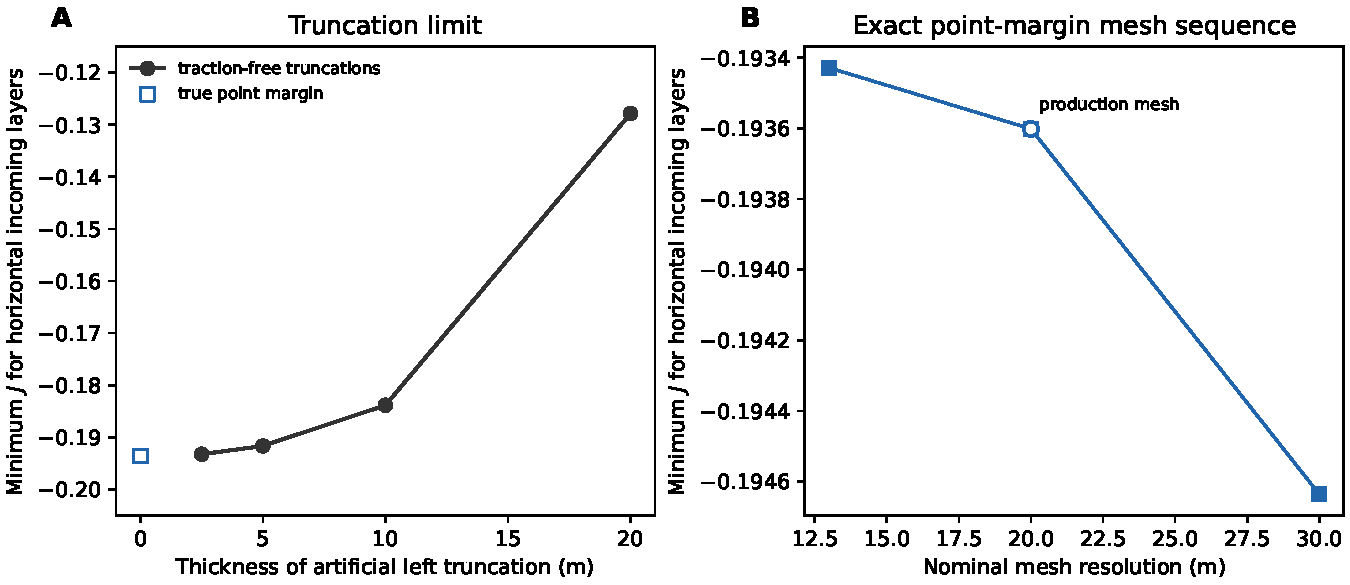
\includegraphics[width=0.92\textwidth]{../figures/allan_hills_nunatak_margin_convergence.pdf}
\caption{Numerical checks for the linear-viscous finite convergent point-margin experiment (\(\eta=2.5\times10^8~\mathrm{Pa\,yr}\)). (a) Minimum \(J\) for horizontal incoming lines as an artificial traction-free left truncation decreases from \(20~\mathrm{m}\) thickness toward the true point margin. (b) Exact point-margin result across three nominal mesh resolutions; the open symbol marks the production mesh used in Figure~\ref{fig:nunatak-margin}. Every value remains negative.}
\label{fig:nunatak-convergence}
\end{figure}

\begin{figure}[h]
\centering
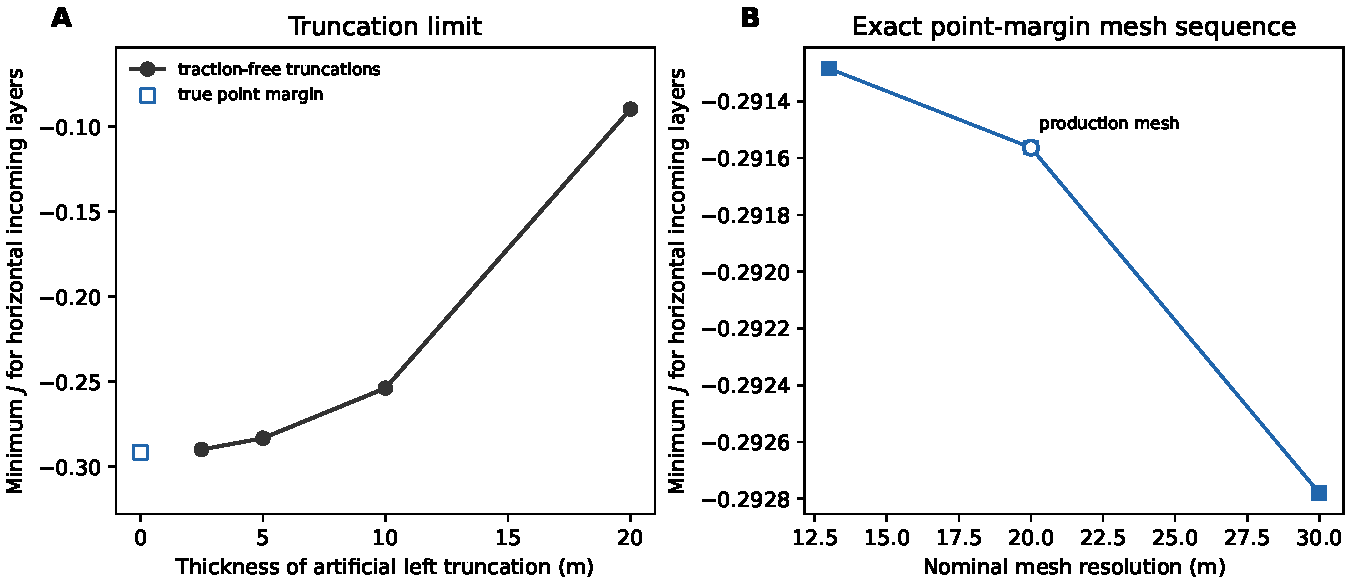
\includegraphics[width=0.92\textwidth]{../figures/allan_hills_nunatak_margin_glen_convergence.pdf}
\caption{Numerical checks for the nonlinear Glen (\(n=3\)) finite convergent point-margin experiment (\(A_{\mathrm{G}}=6.8\times10^{-26}~\mathrm{Pa^{-3}\,s^{-1}}\)). (a) Minimum \(J\) for horizontal incoming lines as an artificial traction-free left truncation decreases from \(20~\mathrm{m}\) thickness (\(-0.0897\)) to \(2.5~\mathrm{m}\) (\(-0.2899\)) toward the true point margin (\(-0.2916\)). (b) Exact point-margin result across the \(30\), \(20\) and \(13~\mathrm{m}\) meshes; the open symbol marks the production mesh used in Figure~\ref{fig:nunatak-margin-glen}. Every value remains negative.}
\label{fig:nunatak-convergence-glen}
\end{figure}

\end{document}
